\documentclass{beamer}

\usepackage{pgfpages}

\mode<presentation>
{
	\usetheme{Boadilla}
	\usecolortheme{dolphin}
	\setbeamertemplate{navigation symbols}{}
	\setbeamerfont{caption}{size=\scriptsize}
}

\mode<handout>
{
	\pgfpagesuselayout{4 on 1}[a4paper,border shrink=5mm,landscape]
	\setbeameroption{show only notes}
	\setbeamerfont{note page}{size=\large}
}

\usefonttheme[onlymath]{serif}
\usepackage{mathpazo}

\usepackage{tikz}
\usepackage{amsmath}
\usepackage{bm}
\usepackage{xspace}
\usetikzlibrary{positioning}
\usetikzlibrary{calc}
\usetikzlibrary{shapes.geometric}
% Useful common abbreviations
\newcommand{\adas}{\textsc{adas}\xspace}
\newcommand{\roi}{\textsc{roi}\xspace}
\newcommand{\eg}{e.g.\xspace}
\newcommand{\ekf}{\textsc{ekf}\xspace}
\newcommand{\klt}{\textsc{klt}\xspace}
\renewcommand{\a}{\r{a}\xspace}
\renewcommand{\aa}{\"a\xspace}
\renewcommand{\o}{\"o\xspace}

% Useful math
\renewcommand{\H}{\bm{H}}
\newcommand{\rotmat}{\bm{\mathcal{R}}}

% Set path to look for figures
\graphicspath{{fig/}}

% Define title page
\title[Vehicle Tracking with Heading Estimation]{Vehicle Tracking with Heading Estimation \\ using a Mono Camera System}
\subtitle{Master's Thesis at Veoneer}
\author{Fredrik Nilsson}
\institute[]{Performed at the Division of Automatic Control \\ Department of Electrical Engineering \\ Link\"oping University}
\date{June 5, 2018}

\begin{document}

\begin{frame}
	\titlepage
	\note
	{
	\begin{itemize}
		\item Presentera dig
		\item Beskriv att exjobbet varit ett samarbete med Veoneer
	\end{itemize}
	}
\end{frame}

\AtBeginSection[]
{
  \begin{frame}{Presentation Outline}
    \tableofcontents[currentsection]
  \end{frame}
}

\begin{frame}{Presentation Outline}
	\tableofcontents
	\note
	{
		\begin{itemize}
			\item G\a igenom agendan f\o{}r presentationen
		\end{itemize}
	}
\end{frame}

% -----------------------------------
\section{Introduction}
% -----------------------------------

\begin{frame}{The Traffic Situation in Sweden}
	\textit{Important traffic statistic from 2017\footnote{Trafikverket, 2018}:}
	\begin{itemize}
		\item Average travelled distance per day with car: 30 km
		\item 4400 people were seriously injured
		\item 253 people were killed
	\end{itemize}
	\pause
	\begin{center}
		\large{According to Euro NCAP, 90 \% of all world-wide traffic \\ accidents are caused by the human factor!}
	\end{center}

	\note
	{
		\begin{itemize}
			\item F\o{}rklara att m\a{}nga m\aa{}nniskor p\a{}verkas av trafiksituationen varje \a{}r i Sverige
		\end{itemize}
	}
\end{frame}

\begin{frame}{Euro NCAP}
	The European New Car Assessment Programme
	\begin{itemize}
		\item Performs vehicle tests and rate car models
		\item Vehicle tests of everyday scenarios, \eg
		\begin{itemize}
			\item Automatic emergency braking for vehicles and pedestrians
			\item Adult and child occupant protection
		\end{itemize}
		\item Puts requirements on the car manufacturers
		\item Higher requirements in the near future!
	\end{itemize}

	\note
	{
		\begin{itemize}
			\item Beskriv kortfattat vad Euro NCAP \aa{}r
			\item Fokusera p\a{} ADAS
		\end{itemize}
	}
\end{frame}

\begin{frame}{Advanced Driver Assistance Systems (\adas)}
	\begin{columns}
	\column{0.6\textwidth}
	\begin{itemize}
		\item An intelligent system to support and help the driver.
		\item Sensors provide information, \eg
		\begin{itemize}
			\item Camera
			\item Radar
			\item LiDAR
		\end{itemize}
		\item Software to process the data and to make decisions
		\item Veoneer (spin-off from Autoliv) is a leading supplier of \adas and autonomous driving.
	\end{itemize}
	\column{0.35\textwidth}
		\begin{figure}
			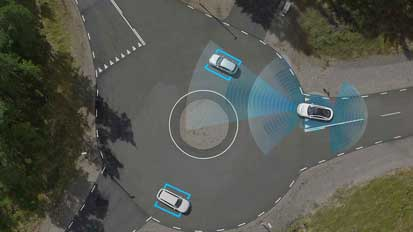
\includegraphics[height=2.25cm]{fig/ALV_Radar-Detection}

			\vspace{0.5em}

			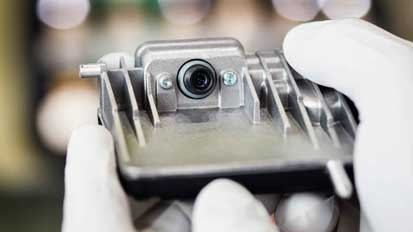
\includegraphics[height=2.25cm]{fig/ALV_Mono-Vision-Sensor}
			\caption{Copyright Autoliv.}
		\end{figure}
	\end{columns}

	\note
	{
		\begin{itemize}
			\item F\o{}rklara vad ett ADAS \aa{}r
			\item Vilken roll har Veoneer?
			\item Relatera till bilderna
		\end{itemize}
	}
\end{frame}

\begin{frame}{Target Tracking in Vision Systems}
	Detect, track and predict the movement of other vehicles.
	\begin{table}
		\centering
		\renewcommand{\arraystretch}{1.25}
		\setlength{\arrayrulewidth}{0.5pt}
		\begin{tabular}{p{5cm}|p{5cm}}
			\textbf{Mono Camera System} & \textbf{Stereo Camera System} \\
			\hline \hline
			Less hardware (1 camera) & More hardware (2 cameras) \\ \hline
            Cheaper & More expensive \\ \hline
			Vehicle detections & Vehicle detections \\ \hline
			No distance information & Distance information \\ \hline
			Difficult to obtain heading information & Easy to obtain heading information
		\end{tabular}
	\end{table}

	\note
	{
		\begin{itemize}
			\item Beskriv kort m\a{}let med target tracking
			\item Skillanderna mellan stereo och mono
			\item \textbf{Fokusera p\a{} kostnaden}
		\end{itemize}
	}
\end{frame}

\begin{frame}{Objective of the Master's Thesis}
	Since depth information is available in the stereo camera, orientation and angular rate are easy to estimate.
	How can we do that in a mono camera system?
	\pause
	\begin{block}{Objective}
		\begin{itemize}
			\item Can the heading (orientation and angular rate) of a vehicle be estimated using a mono camera system?
			\item Which kind of algorithms and models are suitable for solving the problem?
			\item How does a mono camera system performs compared with a stereo camera system?
		\end{itemize}
	\end{block}

	\note
	{
		\begin{itemize}
			\item F\o{}rtydliga att vikten \aa{}r proof-of-concept
		\end{itemize}
	}
\end{frame}

% ------------------------------
\section{Theory and Methodology}
% ------------------------------

\begin{frame}{Method Outline}
	\begin{itemize}
		\item Select a suitable vehicle model
		\item Select and create suitable measurements
		\begin{itemize}
			\item Image detections of the vehicle
			\item Angular rate
			\item Image detections of the vehicle's corners
		\end{itemize}
		\item Construct a filter
		\item Evaluate the performance
		\begin{itemize}
			\item in simulations
			\item with real-world data
		\end{itemize}
	\end{itemize}
\end{frame}

\subsection{Target Tracking}

\begin{frame}{Target Tracking Flow}
	\begin{figure}
	\centering
	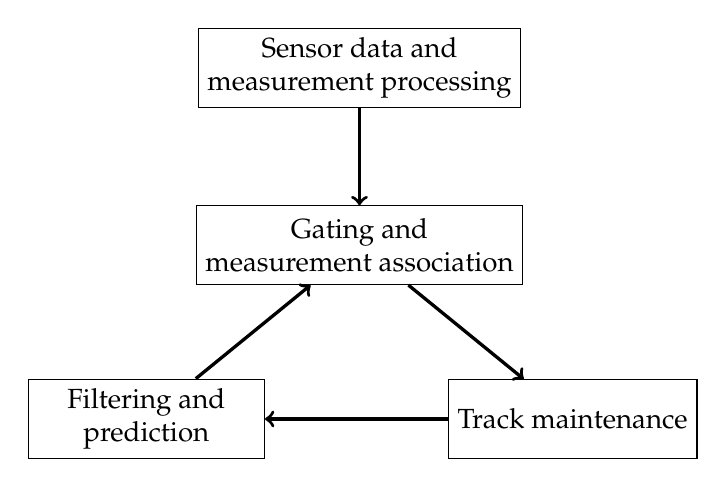
\begin{tikzpicture}
		\tikzstyle{elem} = [rectangle, minimum width = 3cm, minimum height=1cm, align=center, draw=black]

		\node (sensorData) [elem] {Sensor data and \\ measurement processing};
		\node (gatingAssociation) [elem, below of=sensorData, yshift=-1.25cm] {Gating and \\ measurement association};
		\node (trackMaintenance) [elem, below right of=gatingAssociation, yshift=-1.5cm, xshift=2cm] {Track maintenance};
		\node (filter) [elem, below left of=gatingAssociation,  yshift=-1.5cm, xshift=-2cm] {Filtering and \\ prediction};

		\draw [->,very thick] (sensorData) -- (gatingAssociation);
		\draw [->,very thick] (gatingAssociation) -- (trackMaintenance);
		\draw [->,very thick] (trackMaintenance) -- (filter);
		\draw [->,very thick] (filter) -- (gatingAssociation);
	\end{tikzpicture}
	\caption{A flow chart describing a tracking system.}
	\end{figure}

	\note
	{
		\begin{itemize}
			\item \textit{Sensor data and measurement processing}

			Data fr\a{}n sensorer, kan beh\o{}va f\o{}rbehandlas

			\item \textit{Gating and measurement association}

			Logik f\o{}r att avg\o{}ra vilka m\aa{}tningar som \aa{}r m\o{}jliga, associera m\aa{}tningar med m\a{}l

			\item \textit{Track maintenance}

			Skapa nya sp\a{}r, ta bort sp\a{}r, uppdatera logik kring befintliga sp\a{}r

			\item \textit{Filtering and prediction}

			Uppdatera sp\a{}r med m\aa{}tningar och prediktera m\a{}lets r\o{}relse tills n\aa{}sta m\aa{}tning
		\end{itemize}
	}
\end{frame}

\subsection{Feature Points}

\begin{frame}{Feature Points}
	\begin{itemize}
		\item Feature point detection
		\begin{itemize}
			\item Harris corner detector
			\item Shi and Tomasi corner detector
		\end{itemize}
		\item Feature point tracking
		\begin{itemize}
			\item Kanade-Lucas-Tomasi (\klt) feature tracker
		\end{itemize}
	\end{itemize}
	\vspace{-1em}
	\begin{figure}
		\centering
		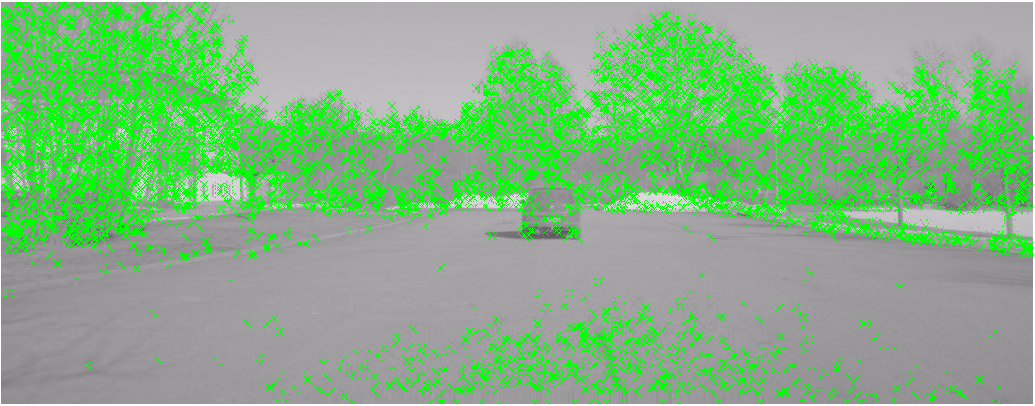
\includegraphics[width=0.75\textwidth]{harris_features}
		\caption{\label{fig:featurepointexample} Detected feature points marked as green crosses.}
	\end{figure}

	\note
	{
		\begin{itemize}
			\item \textit{Detection}

			Olika algoritmer f\o{}r att hitta punkter, bra i olika milj\o{}er

			\item \textit{Description}

			En robust beskrivning av en punkts omgivning.

			\item \textit{Matching}

			Matcha descriptorer extraherade separate i tv\a frames

			\item \textit{Tracking}

			Extrahera punkter i en frame, f\o{}lj sedan dessa frame till frame, \textbf{KLT}
		\end{itemize}
	}
\end{frame}

\subsection{Projective Transformation}

\begin{frame}{Projective Transformation}
	Mapping between different views of the same planar surface,
	\begin{equation*}
		\bm{x}^\prime \sim \H \bm{x},
	\end{equation*}
	where $\H$ is a nonsingular $3 \times 3$ matrix.
	\vspace{1em}
	The \textit{homography} $\H$ can be decomposed into
	\begin{equation*}
		\H = \rotmat + \bm{t} \bm{n}^T.
	\end{equation*}

	\note
	{
		\begin{itemize}
			\item Homografin relaterar hur ett plan har f\o{}rflyttats givet projicerade punkter fr\a{}n planet
			\item Kan delas upp i \textit{rotation} och \textit{translation}
			\item En utmaning -- Inte unik uppdelning (8 till 2 l\o{}sningar)
		\end{itemize}
	}
\end{frame}

\begin{frame}{The Homography -- A Geometrical View}
	\begin{figure}
		\centering
		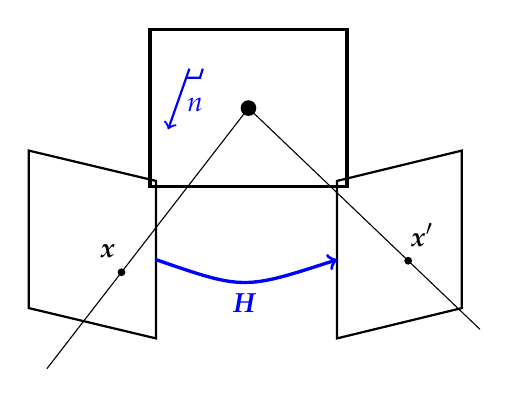
\begin{tikzpicture}
			[plane/.style={very thick,black},
			 image/.style={thick,black},
			 line/.style={black}]

			\draw[plane] (0,0,0) rectangle (2.5,2,0);
			\draw[thick,->,blue] (0.5,1.5,0) -- (1,1.5,2) node[pos=0.6,anchor=west] {$n$};
			\draw[thick,blue] (0.67,1.5,0) -- (0.75,1.5,0.3) -- (0.58,1.5,0.3);

			\draw[image] (0,0,4) -- (0,2,4) -- (2,2,5) -- (2,0,5) -- cycle;
			\draw[image] (4.3,0,5) -- (4.3,2,5) -- (5.5,2,4) -- (5.5,0,4) -- cycle;

			\draw[line] (1.25,1,0) node[circle,fill,inner sep=2pt] {} -- node[label={\hspace{-1em}$\bm{x}$},pos=0.63,circle,fill,inner sep=1pt] {} (1,0,6);
			\draw[line] (1.25,1,0) -- node[label={\hspace{1em}$\bm{x}^\prime$},pos=0.69,circle,fill,inner sep=1pt] {} (6.5,0.5,6);

			\draw[very thick,->,blue] (2,1,5) .. controls (3.5,1,6) .. (4.3,1,5) node[pos=0.5,anchor=north] {$\H$};
		\end{tikzpicture}
		\caption{The homography describing the projective transformation between two views.}
	\end{figure}

	\note
	{
		\begin{itemize}
			\item Ett antagande i min rapport -- Perfekt ego-motion, dvs. stillast\a{}ende host
			\item Homografin inducerats av planets r\o{}relse, dvs. bilens r\o{}relse
		\end{itemize}
	}
\end{frame}

\begin{frame}{Homography for Vehicle Angular Rate}
	\begin{itemize}
		\item Track feature points on the back of the target vehicle
		\item Find the homography between consecutive frames
		\item Decompose and extract the yaw rotation
		\item Calculate the angular rate
	\end{itemize}
	\begin{figure}
		\centering
		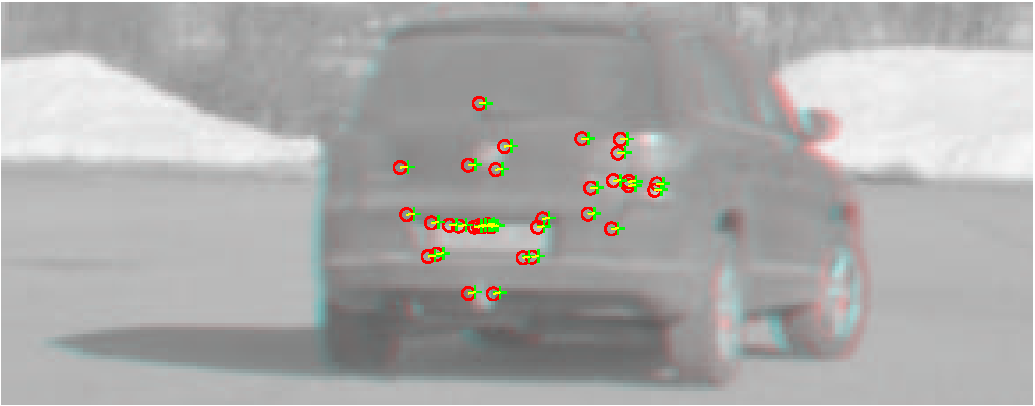
\includegraphics[width=0.8\textwidth]{feature_point_correspondence}
		\caption{Here, feature points have moved from the $1^\text{st}$ frame (red circles) to the $2^\text{nd}$ frame (green crosses).}
	\end{figure}

	\note
	{
		\begin{itemize}
			\item Exempel hur feature punkter har f\o{}rflyttats mellan tv\a frames
		\end{itemize}
	}
\end{frame}

\subsection{Filtering Structure}

\begin{frame}{Filtering Structure}
	\begin{figure}
		\centering
		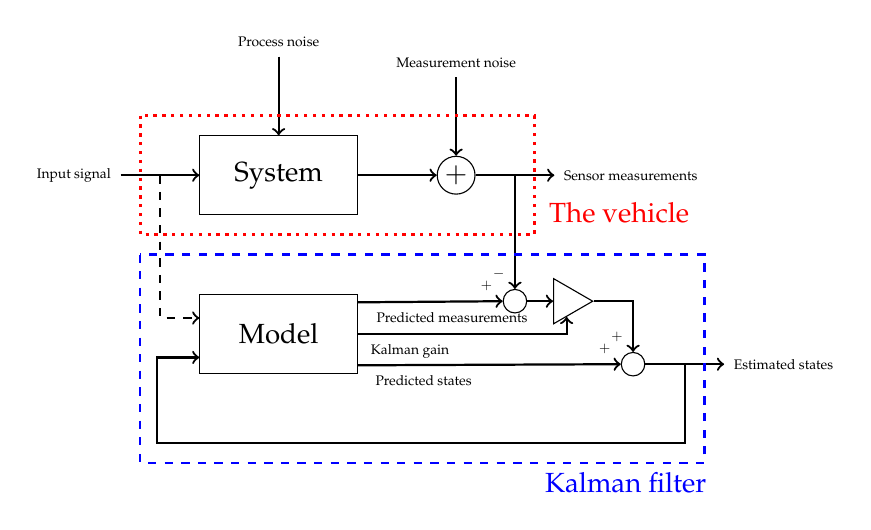
\begin{tikzpicture}
			\tikzstyle{box} = [rectangle, minimum width=2cm, minimum height=1cm, align=center, draw=black]
			\tikzstyle{triangle} = [regular polygon, regular polygon sides=3, align=center, draw=black, shape border rotate=-90]
			\tikzstyle{line} = [thick, black]
			\tikzstyle{sum} = [circle, draw=black, inner sep=1pt]
			\tikzstyle{comb} = [circle, draw=black, inner sep=3pt]

			\node (system)  [box] {System};
			\node (model) [box, below=of system)] {Model};
			\node (sumMeasNoise) [sum, right=of system] {$+$};
			\node (measNoise) [above=of sumMeasNoise] {\tiny Measurement noise};
			\node (procNoise) [above=of system] {\tiny Process noise};
			\node (inputSignal) [left=of system] {\tiny Input signal};
			\node (outputSignal) [right=of sumMeasNoise] {\tiny Sensor measurements};
			\node (combMeas) [comb] at ($(outputSignal.west)+(-0.5,-1.6)$) {};
			\node (combInov) [comb] at ($(combMeas)+(1.5,-0.8)$) {};
			\node (gain) [triangle] at ($(combMeas.east)+(0.5,0)$) {};
			\node (filterOutput) [right=of combInov] {\tiny Estimated states};

			% The system
			\draw[line,->] (procNoise) -- (system);
			\draw[line,->] (inputSignal) -- (system);
			\draw[line,->] (system) -- (sumMeasNoise);
			\draw[line,->] (measNoise) -- (sumMeasNoise);
			\draw[line,->] (sumMeasNoise) -- (outputSignal);

			% The filter
			\draw[line,dashed,->] ($(inputSignal.east)+(0.5,0)$) |- ([yshift=0.3cm]model);
			\draw[line,->] ([yshift=0.4cm]model.east) -- (combMeas.west) node[pos=0.65, anchor=north] {\tiny Predicted measurements} node[anchor=south east] {\tiny $+$};
			\draw[line,->] ($(outputSignal.west)+(-0.5,0)$) -- ($(outputSignal.west)+(-0.5,-0.75)$) -| (combMeas.north) node[anchor=south east] {\tiny $-$};
			\draw[line,->] (combMeas.east) -- (gain);
			\draw[line,->] ([yshift=-0.0cm]model.east) -| (gain.south)  node[pos=0.125, anchor=north] {\tiny Kalman gain};
			\draw[line,->] (gain.east) -| (combInov.north) node[anchor=south east] {\tiny $+$};
			\draw[line,->] ([yshift=-0.4cm]model.east) -- (combInov.west) node[pos=0.25, anchor=north] {\tiny Predicted states} node[anchor=south east] {\tiny $+$};
			\draw[line,->] (combInov) -- (filterOutput);
			\draw[line,->] ([xshift=-0.5cm]filterOutput.west) -- ($(filterOutput.west)+(-0.5,-1)$) -- ($(filterOutput.west)+(-7.2,-1)$) |- ([yshift=-0.3cm]model.west);

			\onslide<2>
			{
			% Surround the filter with a box
			\draw[thick, dashed, blue] ($(model.north west)+(-0.75,0.5)$) rectangle ($([xshift=-0.5cm]filterOutput.west)+(0.25,-1.25)$) node[yshift=-0.25cm,xshift=-1cm] {Kalman filter};
			% Surround the system with a box
			\draw[very thick, dotted, red] ($(system.north west)+(-0.75,0.25)$) rectangle ($([xshift=-0.5cm]outputSignal.west)+(0.25,-0.75)$) node[anchor=south east,xshift=2.1cm] {The vehicle};
			}
		\end{tikzpicture}
	\end{figure}

	\note
	{
		\begin{itemize}
			\item Beskriv signaler till systemet
			\item Beskriv signaler i filtret
		\end{itemize}
	}
\end{frame}

\begin{frame}{Different Image Measurements}
	\begin{figure}
	\centering
	\begin{tikzpicture}
		\node[] at (0,0) {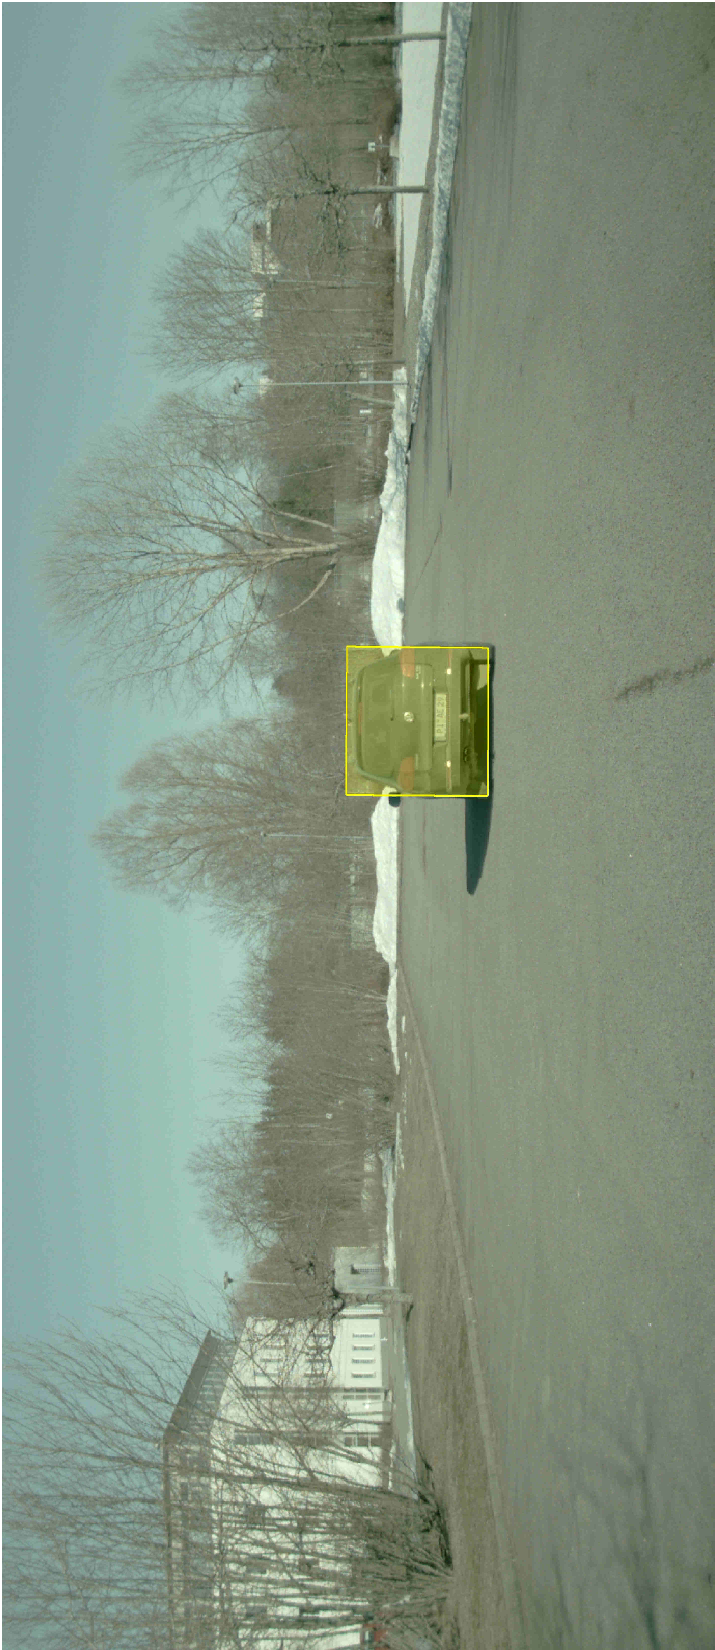
\includegraphics[angle=-90,origin=c,trim={0 0 15cm 0},width=0.45\textwidth]{roi_example}};
		\draw[red, thick, |->] (0,-0.38) -- (0.35,-0.38) node[anchor=north] {\tiny $p_\text{HCP}$};
	\end{tikzpicture}
	\begin{tikzpicture}
		\node[] at (0,0) {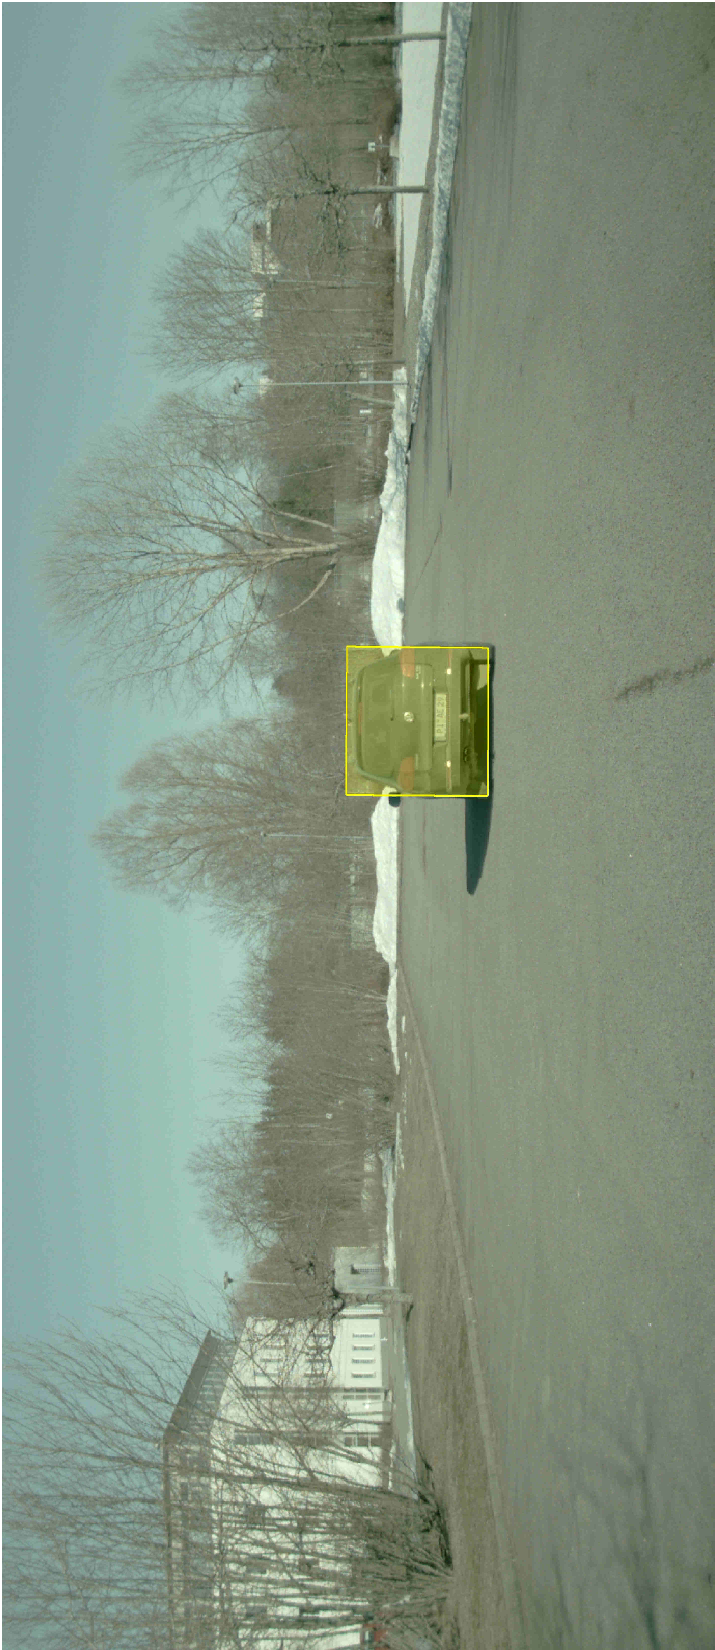
\includegraphics[angle=-90,origin=c,trim={0 0 15cm 0},width=0.45\textwidth]{roi_example}};
		\draw[red, thick, <->] (0.08,0.075) -- (0.6,0.075) node[pos = 0.5, anchor=south] {\tiny $p_\text{Width}$};
	\end{tikzpicture}

	\begin{tikzpicture}
		\node[] at (0,0) {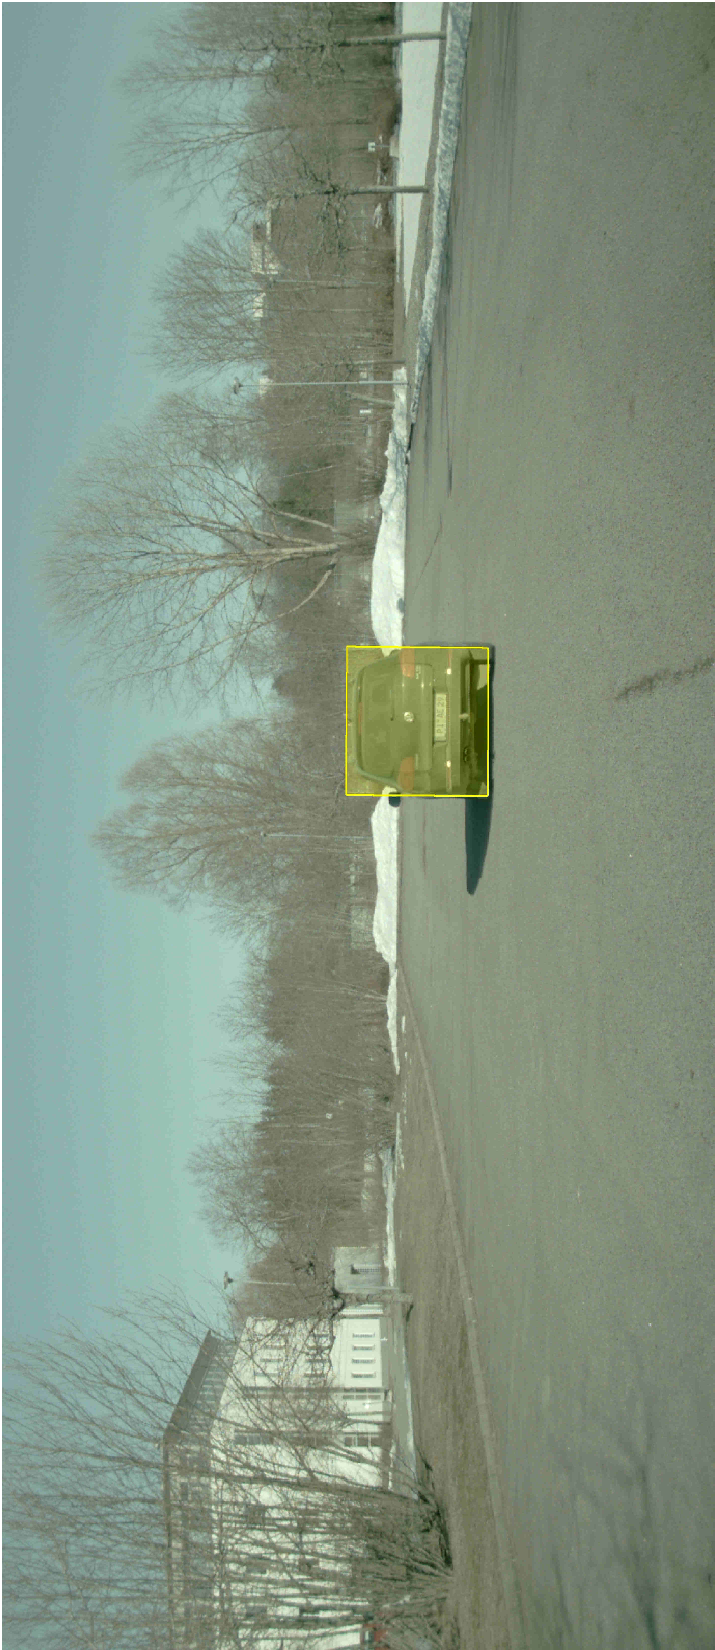
\includegraphics[angle=-90,origin=c,trim={0 0 15cm 0},width=0.45\textwidth]{roi_example}};
		\draw[red, thick, |->] (0.35,0) -- (0.35,-0.39) node[pos = 0.5, anchor=west] {\tiny $p_\text{Bottom}$};
	\end{tikzpicture}
	\begin{tikzpicture}
		\node[] at (0,0) {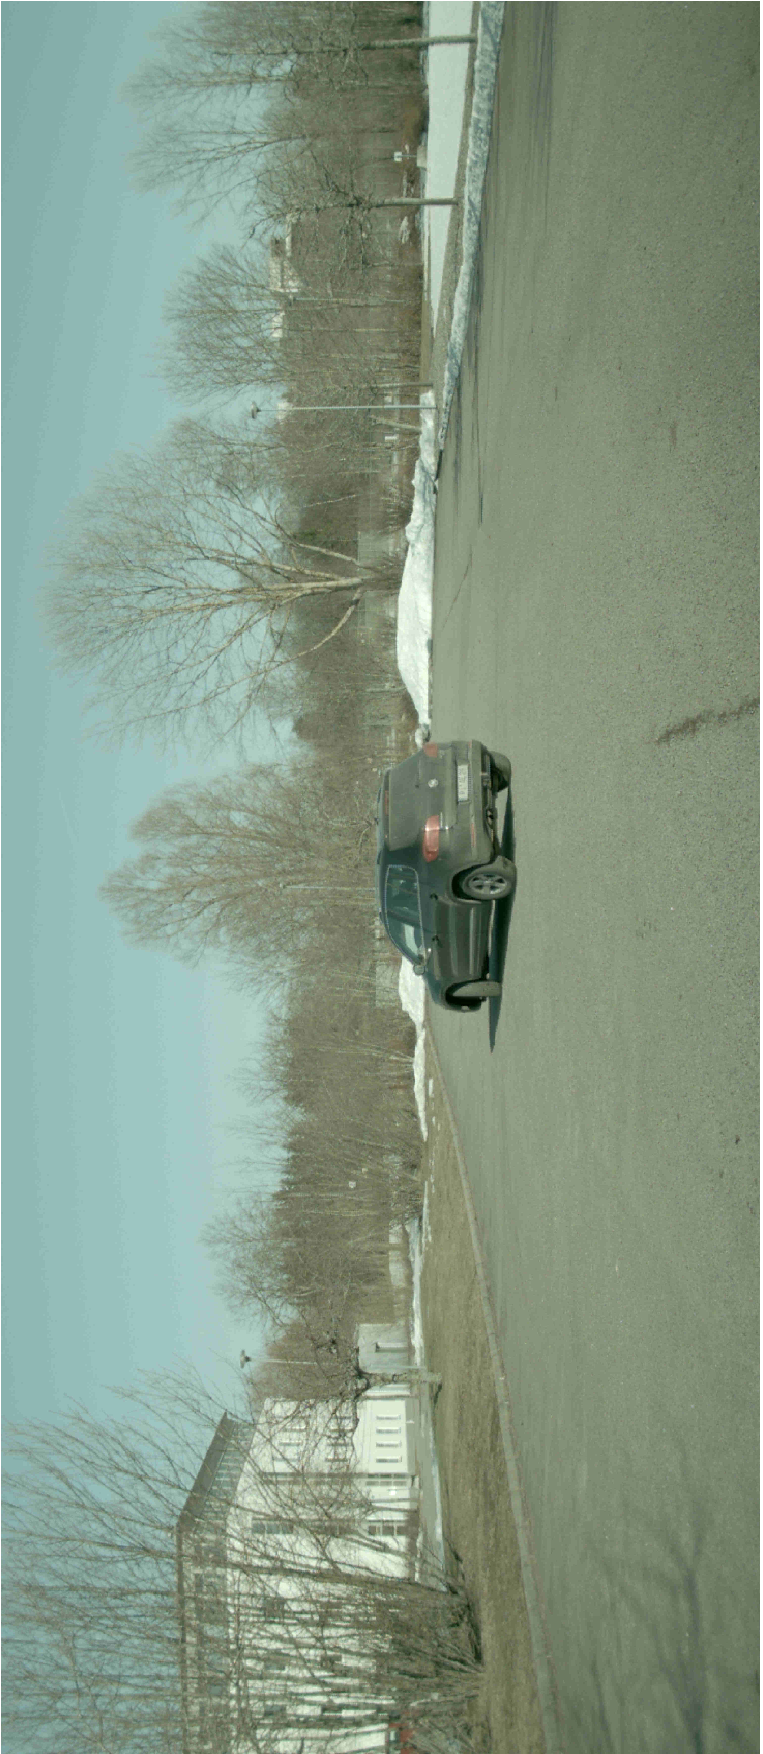
\includegraphics[angle=-90,origin=c,trim={0 0 16cm 0},width=0.45\textwidth]{corners_example}};
		\node[red,circle,fill,inner sep=0.75pt,label=left:{\color{red}\tiny FL}] at (-0.4,-0.325) {};
		\node[red,circle,fill,inner sep=0.75pt,label=below:{\color{red}\tiny RL}] at (0.07,-0.4) {};
		\node[red,circle,fill,inner sep=0.75pt,label=right:{\color{red}\tiny RR}] at (0.4,-0.37) {};
	\end{tikzpicture}
	\caption{The different image measurements used in the filter.}
	\end{figure}

	\note
	{
		\begin{itemize}
			\item Machine learning-algoritm tr\aa{}nad f\o{}r att detektera bilar
			\item H\o{}rnm\aa{}tningarna finns det inget detektor f\o{}r idag
		\end{itemize}
	}
\end{frame}

\begin{frame}{Summary of the Filter Structure}
	\begin{columns}
	\column{0.6\textwidth}
		\begin{itemize}
			\item Vehicle modelled as a rectangle
			\item An extended Kalman filter (\ekf)
			\item A constant velocity motion model
			\item State vector $\bm{x}=\begin{pmatrix} x & y & z & v & \psi & \omega \end{pmatrix}^T$
			\item The position and orientation are relative to the ego vehicle
		\end{itemize}
	\column{0.4\textwidth}
		\begin{figure}
			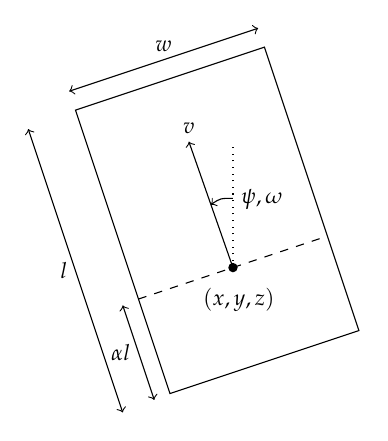
\begin{tikzpicture}[scale=0.8, every node/.style={scale=0.8}]
				\draw (0,0) -- (3,1) -- (1.5,5.5) -- (-1.5,4.5) -- cycle;
				\draw[dashed] (-0.5,1.5) -- (2.5,2.5) node[pos=0.3, anchor=north west] {$(x,y,z)$};
				\draw[->] (1,2) node[circle,fill,inner sep=1.5pt] {} -- (0.3,4) node[anchor=south] {$v$};
				\draw[dotted] (1,2) -- (1,4);
				\draw[<-] (0.65,3) .. controls (0.8,3.1) .. (1,3.1) node[pos=0.5, anchor=west] {\hspace{0.2cm}$\psi, \omega$};
				\draw[<->] (-0.25,-0.1) -- (-0.75,1.4) node[pos=0.5, anchor=east] {$\alpha l$};
				\draw[<->] (-0.75,-0.3) -- (-2.25,4.2) node[pos=0.5, anchor=east] {$l$};
				\draw[<->] (-1.6,4.8) -- (1.4,5.8) node[pos=0.5, anchor=south] {$w$};
		    \end{tikzpicture}
		    \caption{Target vehicle model.}
		\end{figure}
	\end{columns}

	\note
	{
		\begin{itemize}
			\item Rektangel naturlig modell
			\item Enkelt att definiera rotationen och anpassad till h\o{}rnm\aa{}tningarna
			\item M\a{}let \aa{}r att skatta $\phi$ och $\omega$
			\item Till\a{}nden $x, y, z$ och $v$ kommer naturligt med
		\end{itemize}
	}
\end{frame}

\subsection<presentation:0>
{Observability}

\begin{frame}<presentation:0>[noframenumbering]
	\frametitle{Nonlinear Observability}
	\begin{itemize}
		\item In general, it is difficult to prove observability for nonlinear system.
		\begin{align*}
			\bm{x}_{k+1} &= \bm{f}(\bm{x}_k), \\
			\bm{y}_k &= \bm{h}(\bm{x}_k).
		\end{align*}
		\item The observability Gramian matrix, $\bm{M}$, can be calculated as
		\begin{equation*}
			\bm{M}(t_0,t_N) = \sum_{j=t_0}^{t_N-1} \bm{\Phi}^T(j,t_0)\bm{H}^T_j\bm{H}_j\bm{\Phi}(j,t_0),
		\end{equation*}
		where $\bm{\Phi}$ is the transition matrix (of the linearized system) and $\bm{H}$ is the Jacobian of $\bm{h}$.
		\item The trajectory is observable on $[t_0, t_N]$ if the observability Gramian matrix is invertible.
	\end{itemize}

	\note
	{
		\begin{itemize}
			\item Eftersom Jacobianen f\o{}r\aa{}ndras f\o{}r varje enskild trajektoria \aa{}r det sv\a{}rt att dra n\a{}gra generella slutsatser
			\item Dock kan det ge en fingervisning
		\end{itemize}
	}
\end{frame}

% ---------------
\section{Results}
% ---------------

\note
{
	\begin{itemize}
		\item \textit{Simulated Results}

		Monte Carlo simuleringar av tv\a{} fall, bed\o{}ma prestanda, \textbf{variera brusniv\a{}er}

		\item \textit{Homography Estimation}

		Hur bra \a{}r min metod f\o{}r att skatta homografier, simulerad rektangel (baksidan av en bil)

		\item \textit{Stereo Comparison}

		Ett av m\a{}len, j\aa{}mf\o{}ra med ett stereo kamera system
	\end{itemize}
}

\subsection<presentation:0>
{Observability}

\begin{frame}<presentation:0>[noframenumbering]
	\frametitle{Observability Results}
	\begin{table}
		\centering
		\scriptsize
		\renewcommand{\arraystretch}{1.25}
		\setlength{\arrayrulewidth}{0.5pt}
		\begin{tabular}{|p{5cm}|p{1cm}|p{2.1cm}|p{2.1cm}|}
			\cline{2-4}
			\multicolumn{1}{c|}{} & \multicolumn{3}{c|}{\textbf{Observable}} \\
			\hline
			\textbf{Description} & \roi & \roi and angular rate & \roi, angular rate and corners \\
			\hline
			\hline
			The target is standing still with an arbitrary initial yaw angle. & No & No & Yes \\
			\hline
			The target is driving straight towards or straight away from the host. & Yes & Yes & Yes \\
			\hline
			The target is driving towards or away from the host applying sine steering. & Yes & Yes & Yes \\
			\hline
			The target is driving away from the host and makes a $45^\circ$ turn. & Yes & Yes & Yes \\
			\hline
			The target is driving across the host's lane with constant speed and constant yaw angle. & Yes & Yes & Yes \\
			\hline
		\end{tabular}
	\end{table}

	\note
	{
		\begin{itemize}
			\item Om m\a{}let st\a{}r stilla, s\a{} finns det flera tillst\a{}ndsvektorer som ger samma \roi.
		\end{itemize}
	}
\end{frame}

\subsection{Monte Carlo Simulations}

\begin{frame}{Monte Carlo Simulations -- No. 1}
	The target is driving straight.
	\vspace{2em}
	\begin{columns}
	\column{0.45\textwidth}
	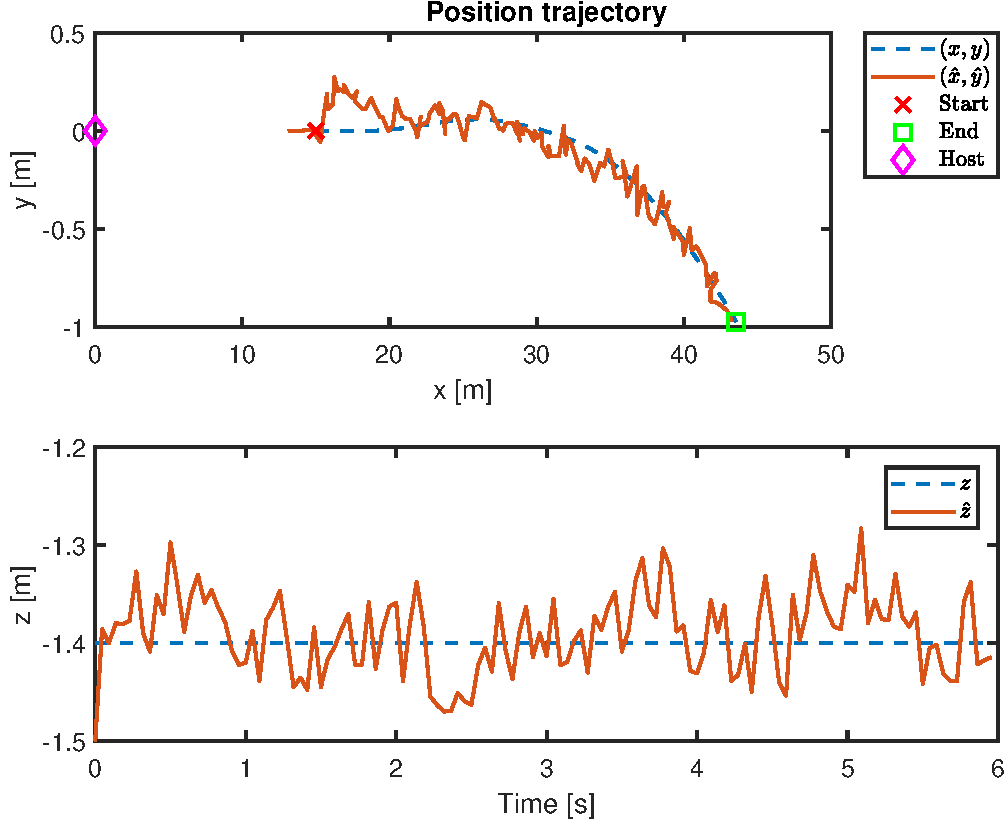
\includegraphics[width=\textwidth]{Traj/20_MC_TrajPos}
	\column{0.45\textwidth}
	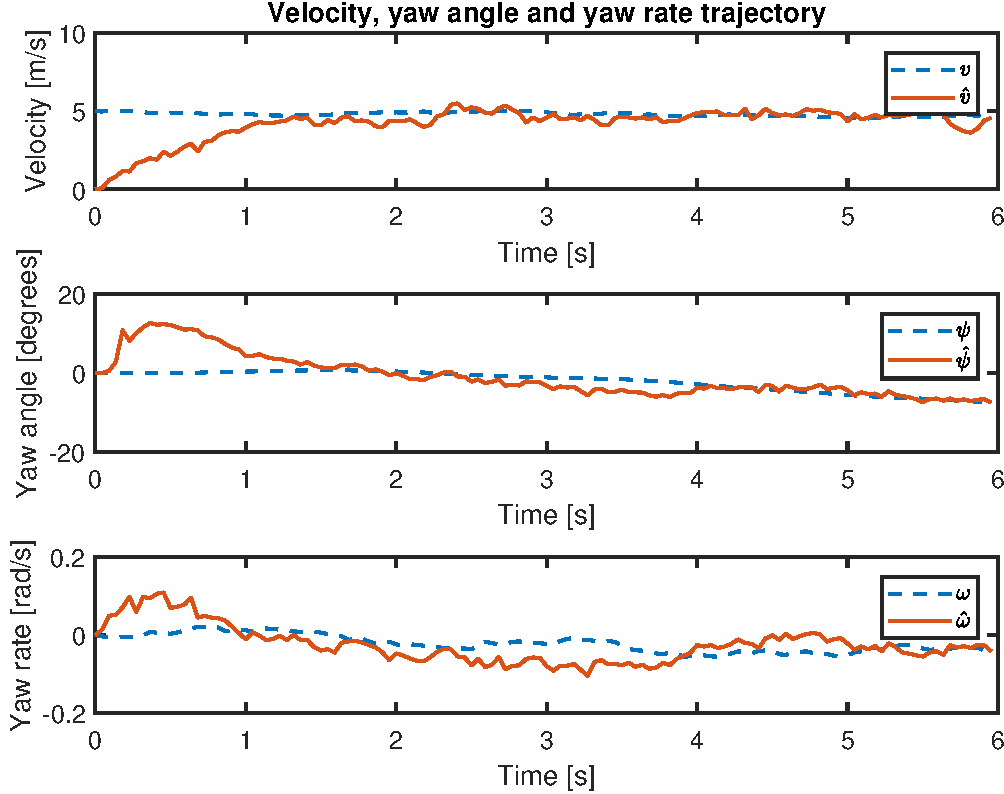
\includegraphics[width=\textwidth]{Traj/20_MC_TrajOther}
	\end{columns}

	\note
	{
		\begin{itemize}
			\item Targetbil som k\o{}r rakt fram
			\item Konstant hastighet
			\item Ingen rotation
		\end{itemize}
	}
\end{frame}

\begin{frame}{Monte Carlo Results -- No. 1}
	\begin{columns}[T]
	\column{0.45\textwidth}
	\begin{figure}
		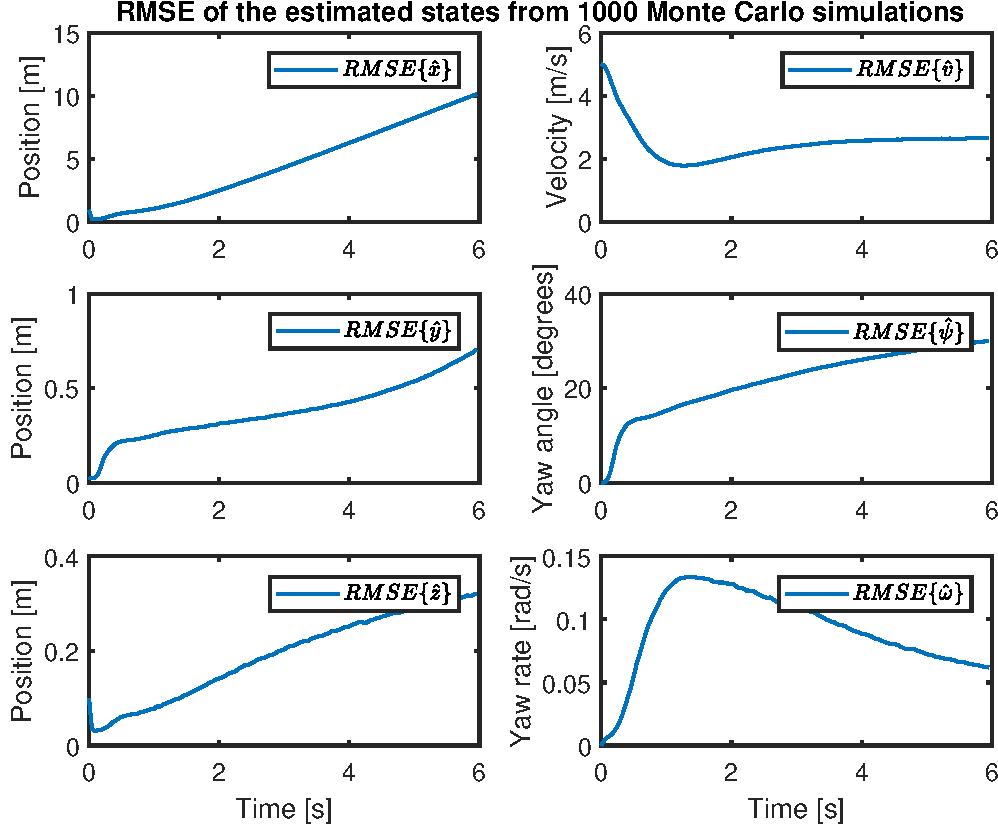
\includegraphics[width=\textwidth]{MC/27_MC_1000_Rmse}
		\caption{Only \roi measurements.}
	\end{figure}
	\column{0.45\textwidth}
	\begin{figure}
		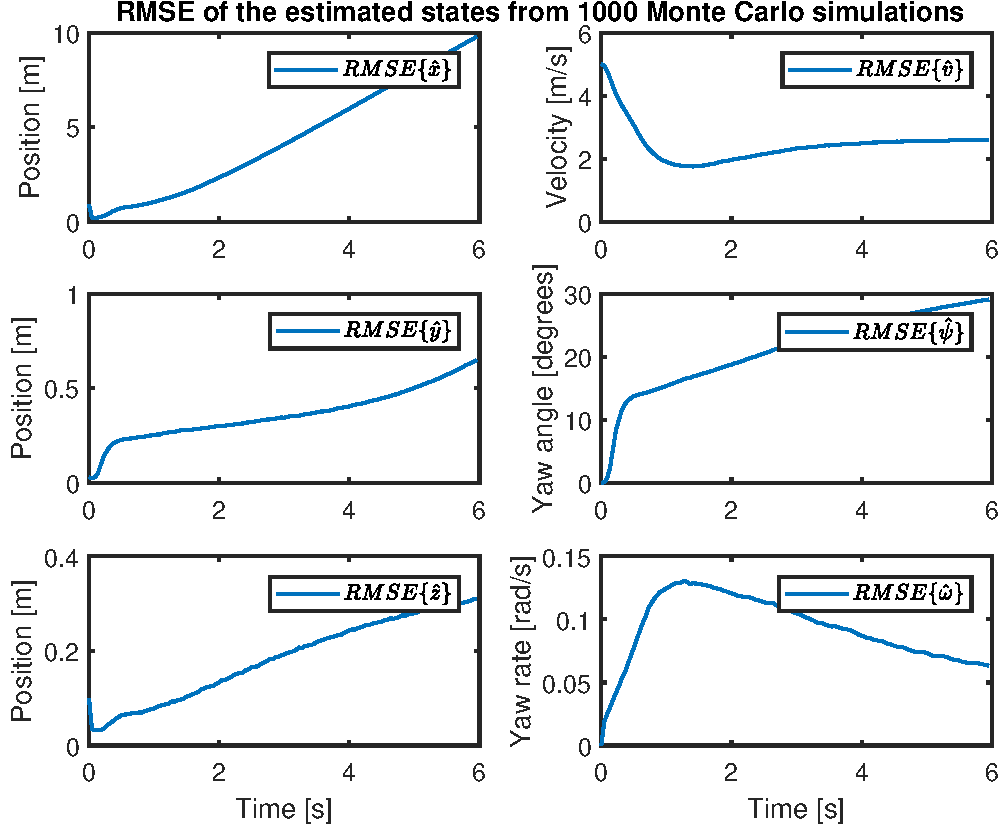
\includegraphics[width=\textwidth]{MC/22_MC_1000_Rmse}
		\caption{\roi and angular rate (with noise variance 1 rad/s) measurements.}
	\end{figure}
	\end{columns}

	\note
	{
		\begin{itemize}
			\item Visar felet mellan skattade och sanna tillst\a{}nd
			\item H\aa{}r ger vinkelhastighetsm\aa{}tningarna ingen information
		\end{itemize}
	}
\end{frame}

\begin{frame}{Monte Carlo Results -- No. 1}
	\begin{columns}[T]
	\column{0.45\textwidth}
	\begin{figure}
		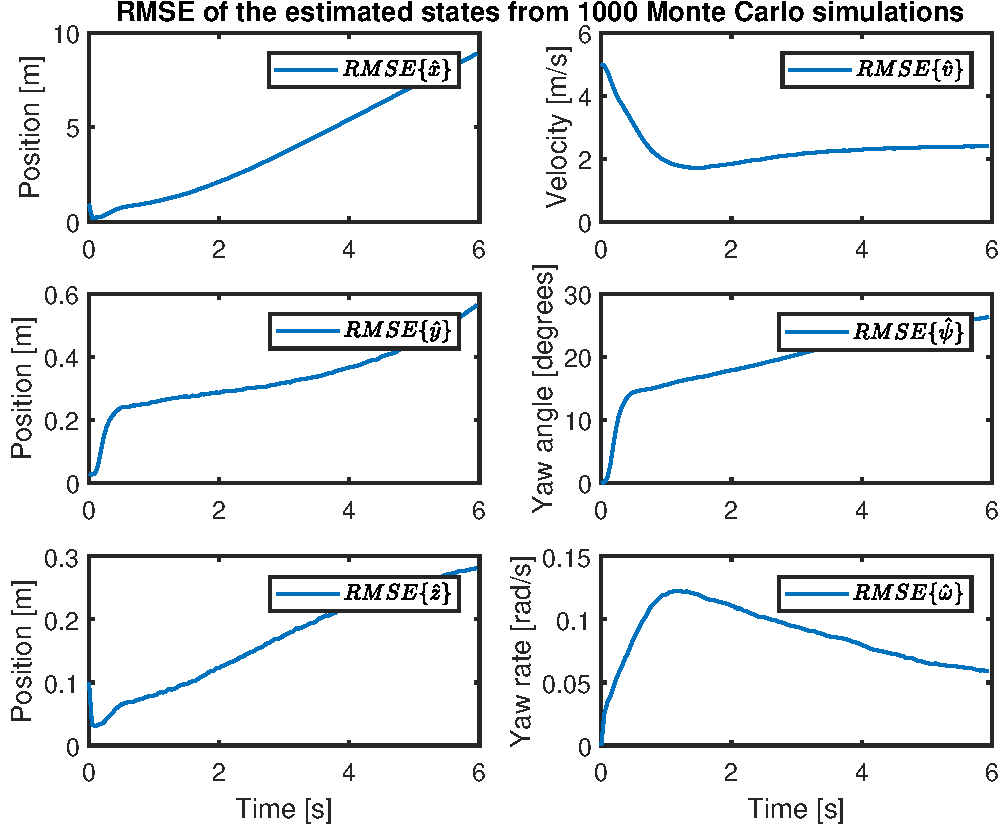
\includegraphics[width=\textwidth]{MC/21_MC_1000_Rmse}
		\caption{\roi and angular rate (with noise variance 0.5 rad/s) measurements.}
	\end{figure}
	\column{0.45\textwidth}
	\begin{figure}
		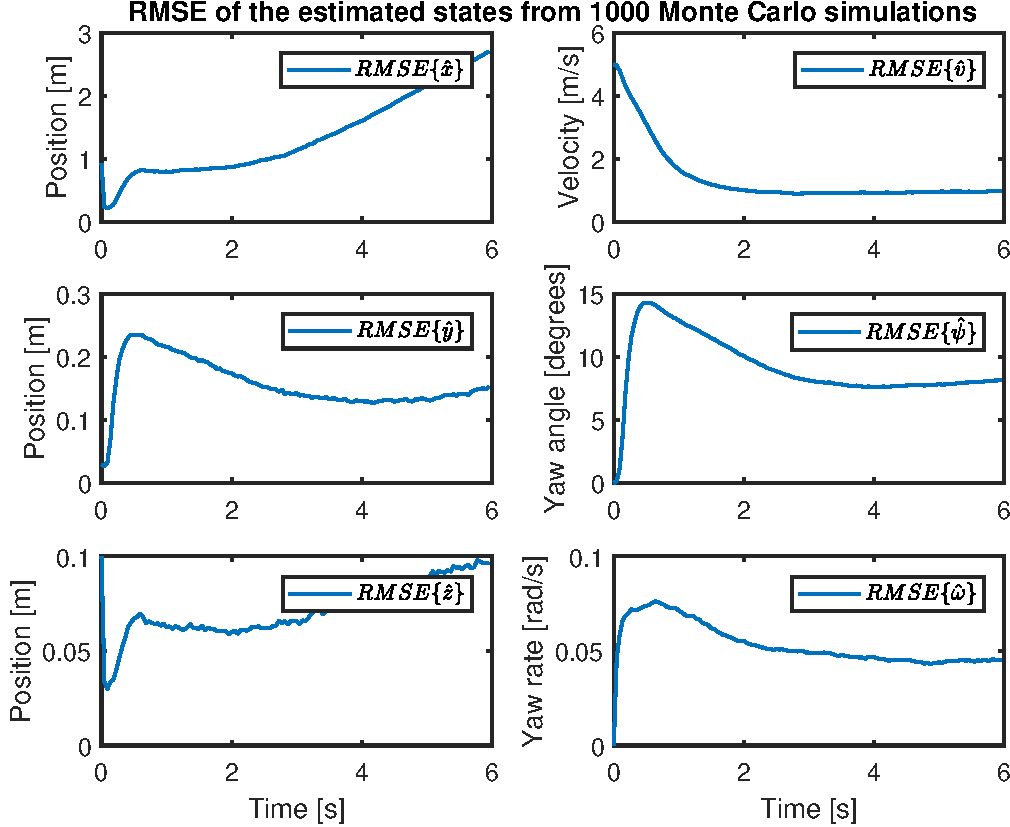
\includegraphics[width=\textwidth]{MC/20_MC_1000_Rmse}
		\caption{\roi and angular rate (with noise variance 0.1 rad/s) measurements.}
	\end{figure}
	\end{columns}

	\note
	{
		\begin{itemize}
			\item Om tillr\aa{}kligt l\a{}gt brus ger vinkelhastighetsm\aa{}tningarna bra information
			\item Fokusera p\a{} orientering och vinkelhastighet
		\end{itemize}
	}
\end{frame}

\begin{frame}{Monte Carlo Simulations -- No. 2}
	The target is turning to the right.
	\vspace{1em}
	\begin{columns}
	\column{0.45\textwidth}
	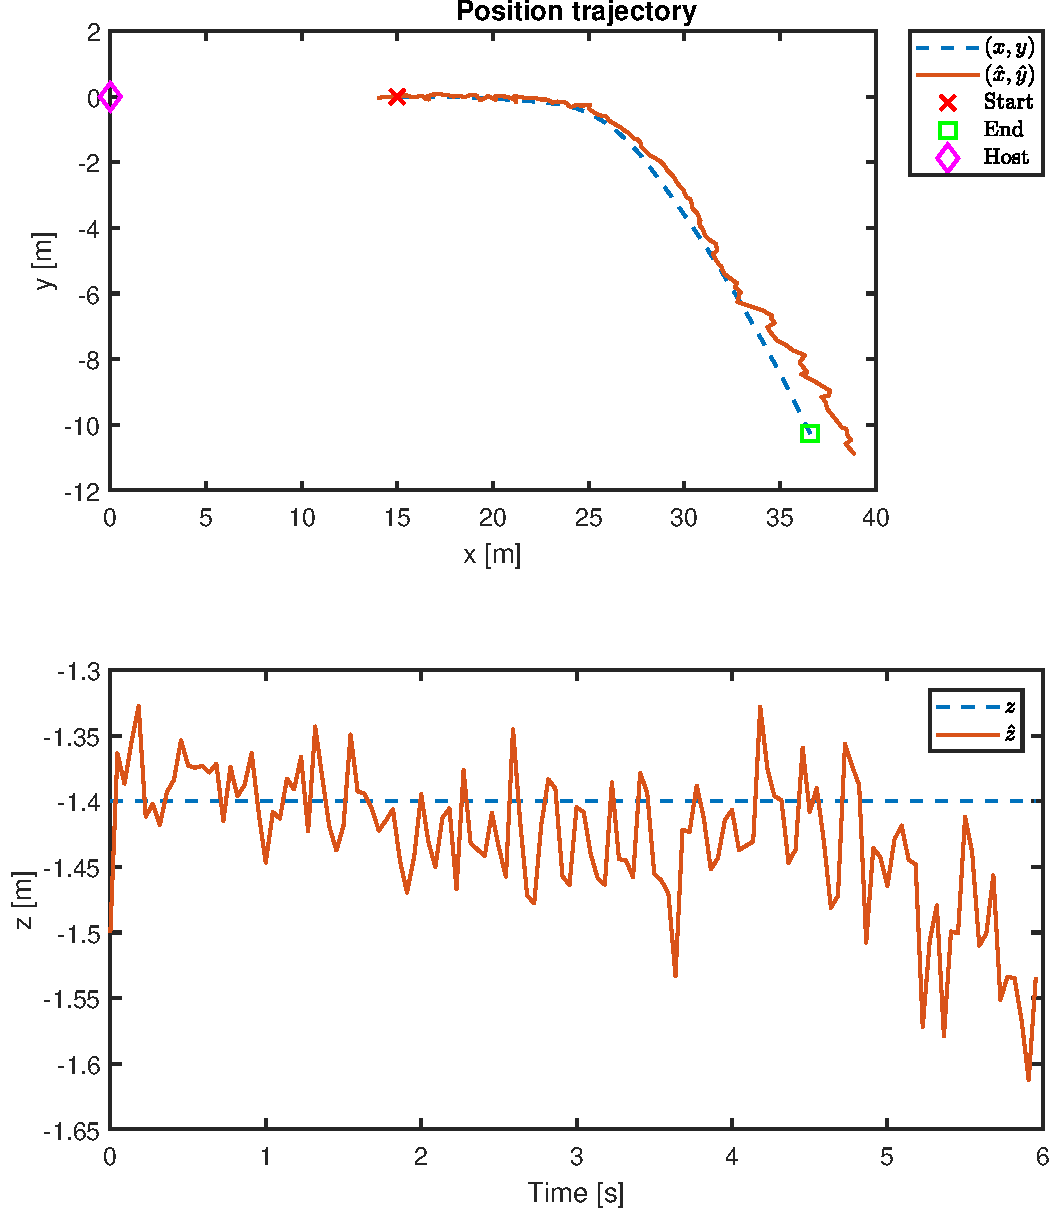
\includegraphics[width=\textwidth]{Traj/23_MC_TrajPos}
	\column{0.45\textwidth}
	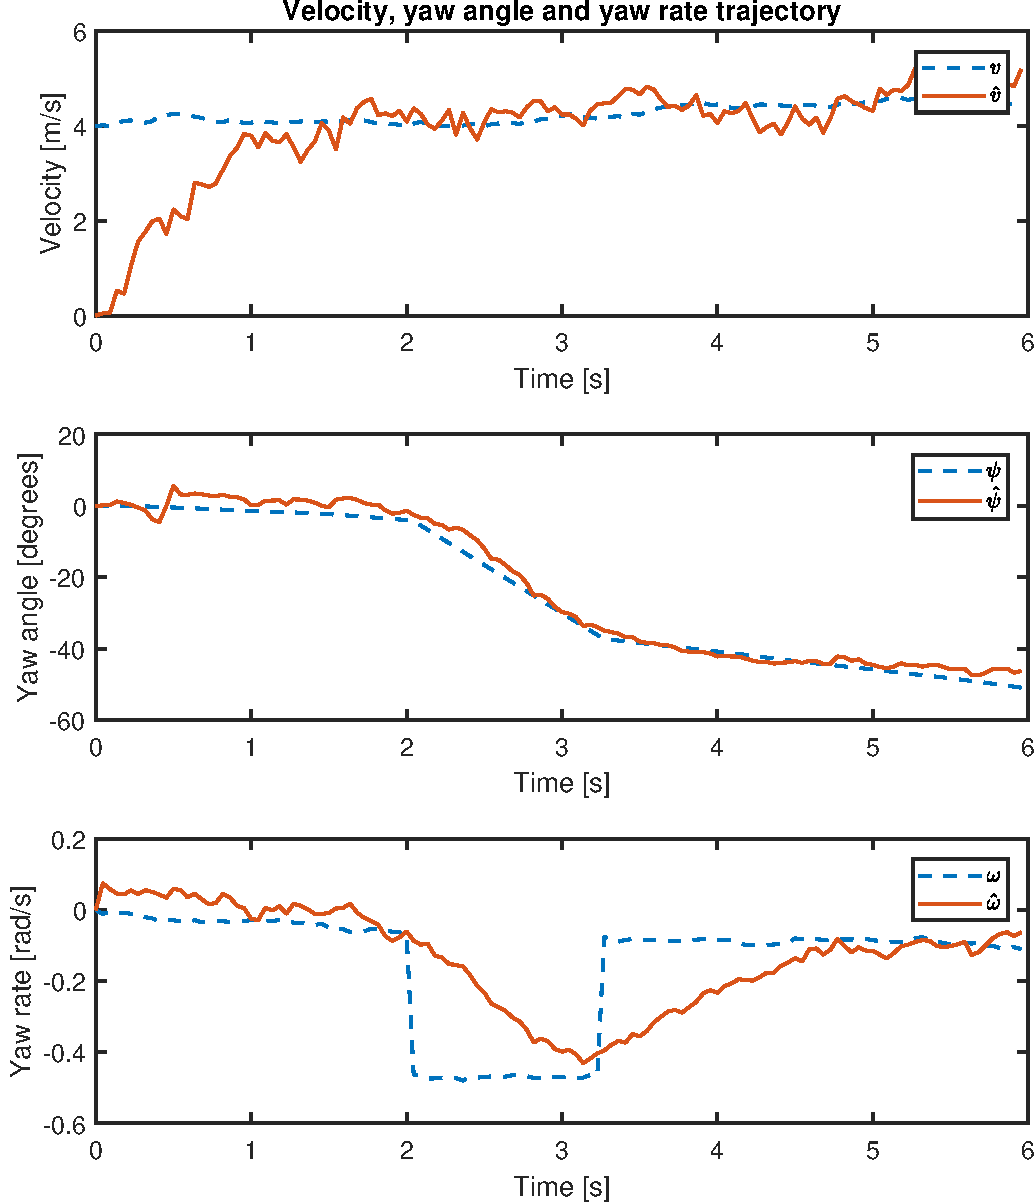
\includegraphics[width=\textwidth]{Traj/23_MC_TrajOther}
	\end{columns}

	\note
	{
		\begin{itemize}
			\item Targetbil som k\o{}r rakt och sv\aa{}nger sedan till h\o{}ger
			\item Konstant hastighet
			\item Tonstant rotationshastighet under sv\aa{}ngen
		\end{itemize}
	}
\end{frame}

\begin{frame}{Monte Carlo Results -- No. 2}
	\begin{columns}[T]
	\column{0.45\textwidth}
	\begin{figure}
		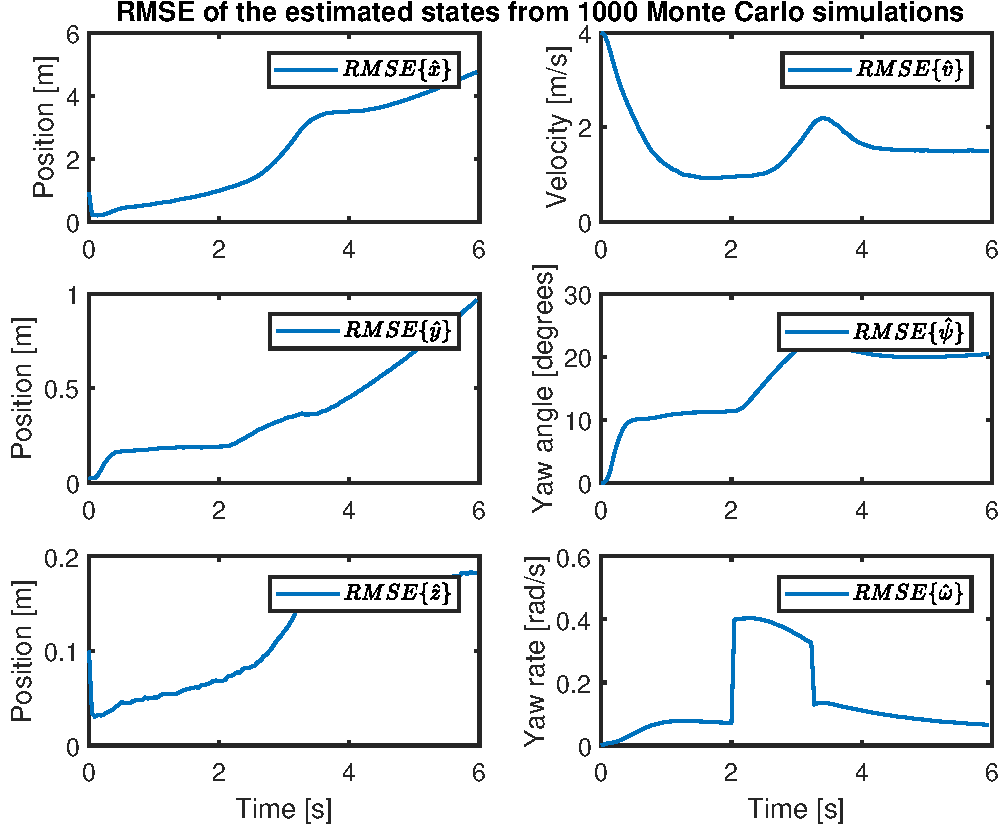
\includegraphics[width=\textwidth]{MC/13_MC_1000_Rmse}
		\caption{Only \roi measurements.}
	\end{figure}
	\column{0.45\textwidth}
	\begin{figure}
		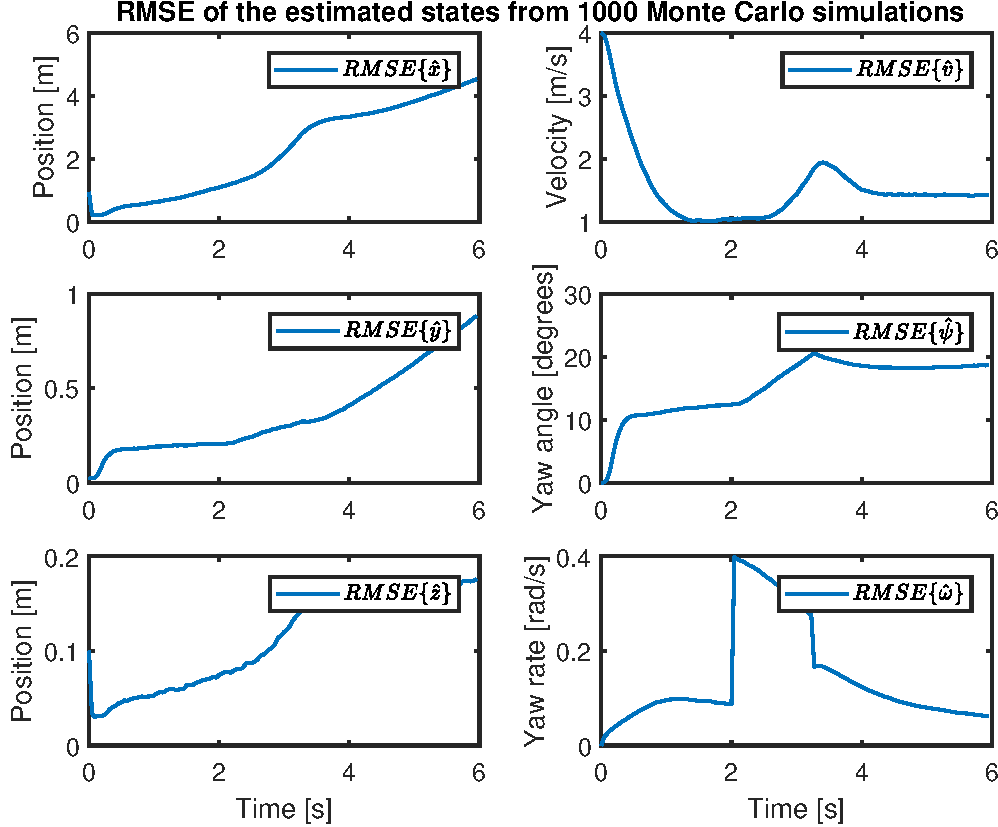
\includegraphics[width=\textwidth]{MC/25_MC_1000_Rmse}
		\caption{\roi and angular rate (with noise variance 1 rad/s) measurements.}
	\end{figure}
	\end{columns}

	\note
	{
		\begin{itemize}
			\item Visar felet mellan skattade och sanna tillst\a{}nd
			\item H\aa{}r ger vinkelhastighetsm\aa{}tningarna ingen information
		\end{itemize}
	}
\end{frame}

\begin{frame}{Monte Carlo Results -- No. 2}
	\begin{columns}[T]
	\column{0.45\textwidth}
	\begin{figure}
		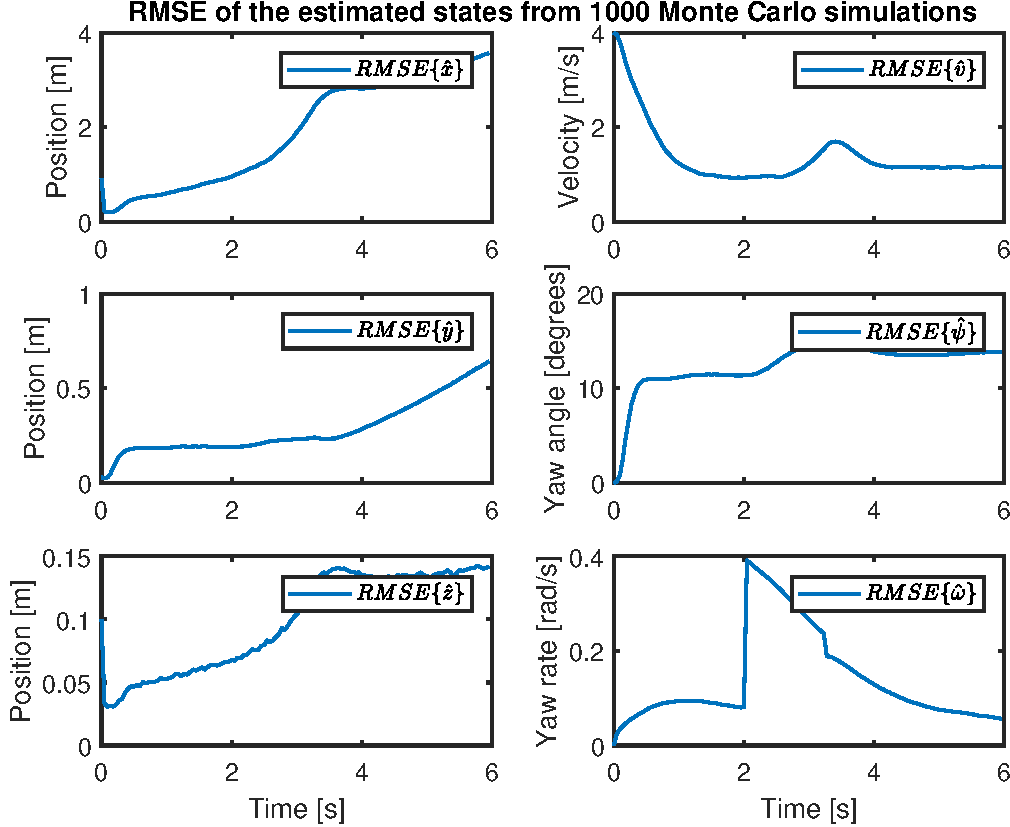
\includegraphics[width=\textwidth]{MC/24_MC_1000_Rmse}
		\caption{\roi and angular rate (with noise variance 0.5 rad/s) measurements.}
	\end{figure}
	\column{0.45\textwidth}
	\begin{figure}
		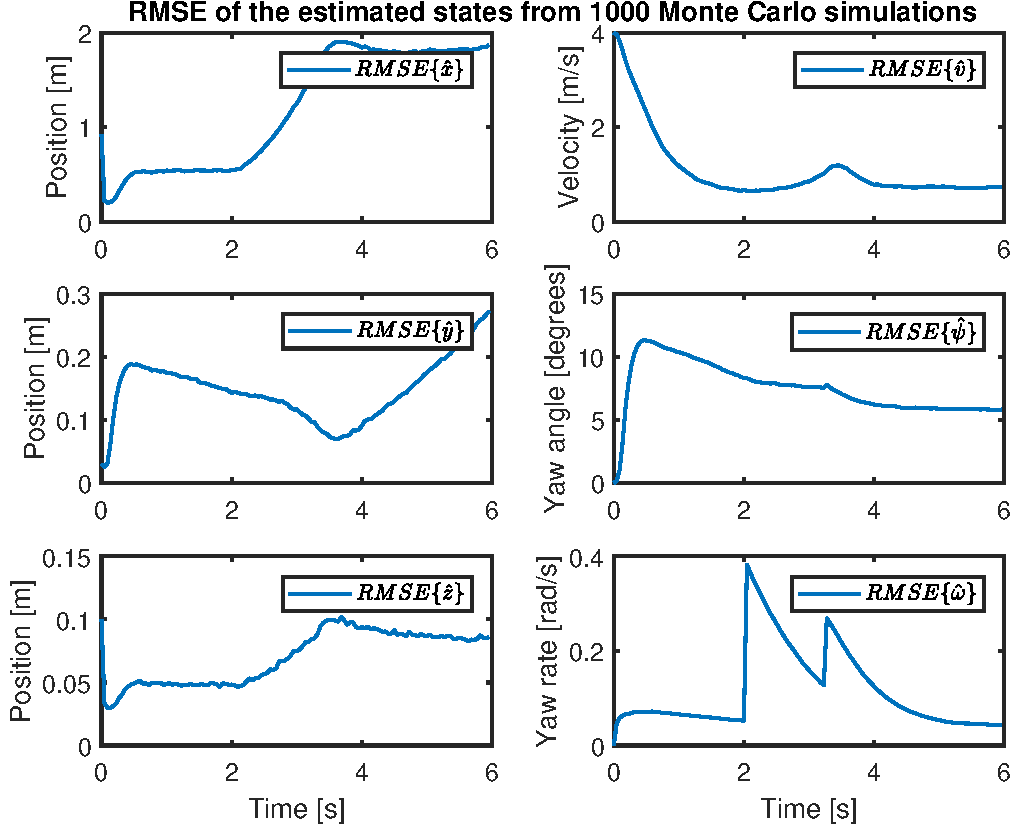
\includegraphics[width=\textwidth]{MC/23_MC_1000_Rmse}
		\caption{\roi and angular rate (with noise variance 0.1 rad/s) measurements.}
	\end{figure}
	\end{columns}

	\note
	{
		\begin{itemize}
			\item Om tillr\aa{}kligt l\a{}gt brus ger vinkelhastighetsm\aa{}tningarna bra information
			\item Fokusera p\a{} orientering och vinkelhastighet
		\end{itemize}
	}
\end{frame}

\begin{frame}{Monte Carlo Results with Corner Measurements}
	\begin{columns}[T]
	\column{0.45\textwidth}
	Driving straight (no. 1):
	\begin{figure}
		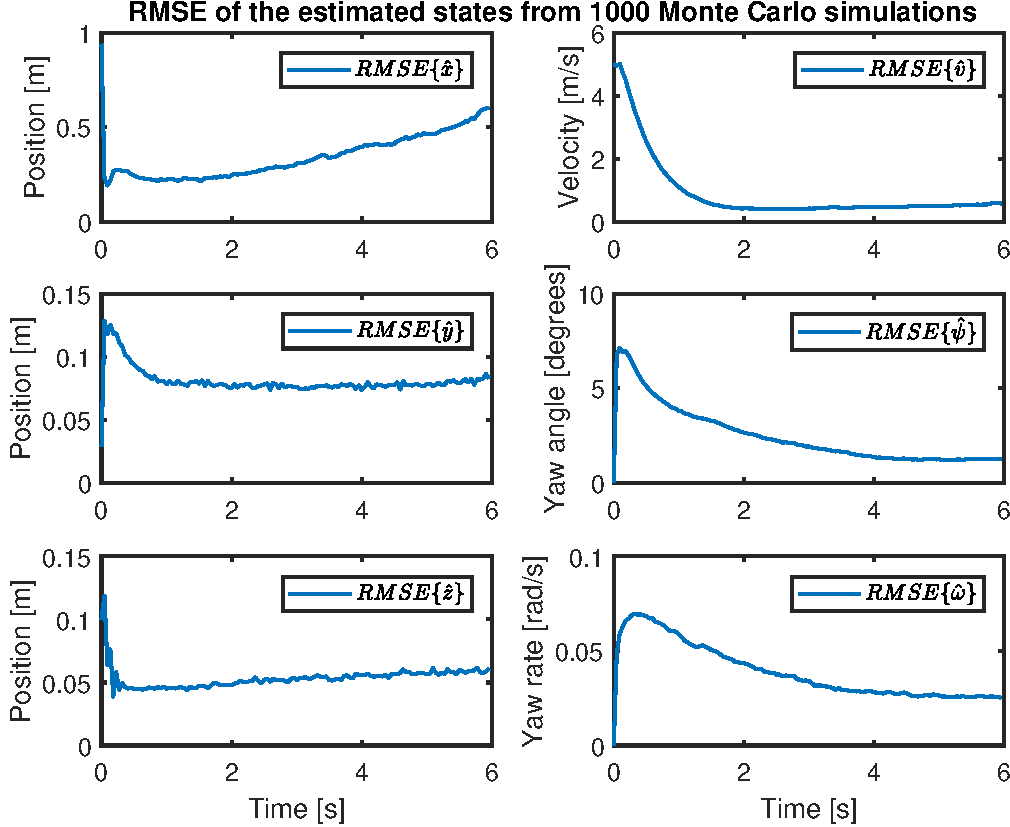
\includegraphics[width=\textwidth]{MC/30_MC_1000_Rmse}
		\caption{\roi, angular rate and corner measurements.}
	\end{figure}
	\column{0.45\textwidth}
	Turning right (no. 2):
	\begin{figure}
		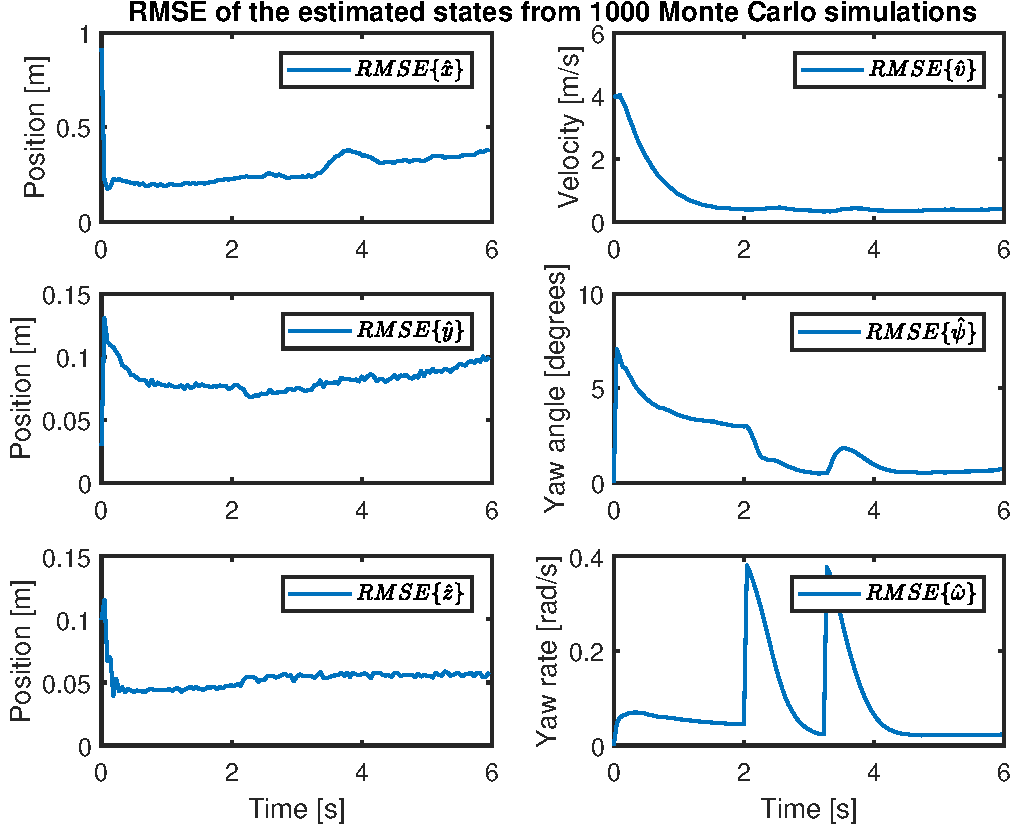
\includegraphics[width=\textwidth]{MC/29_MC_1000_Rmse}
		\caption{\roi, angular rate and corner measurements.}
	\end{figure}
	\end{columns}

	\note
	{
		\begin{itemize}
			\item Stor prestandaf\o{}rb\aa{}ttring om h\o{}rnm\aa{}tningar hade funnits
			\item B\aa{}ttre prestanda vid sv\aa{}ng -- 3 h\o{}rn synliga
		\end{itemize}
	}
\end{frame}

\subsection{Homography Estimation}

\begin{frame}{Homography Estimation Results -- Simulations}
	Simulation of a moving rectangle with different Gaussian noise realisations.
	\vspace{-1.5em}
	\begin{columns}[T]
	\column{0.45\textwidth}
	\begin{figure}
		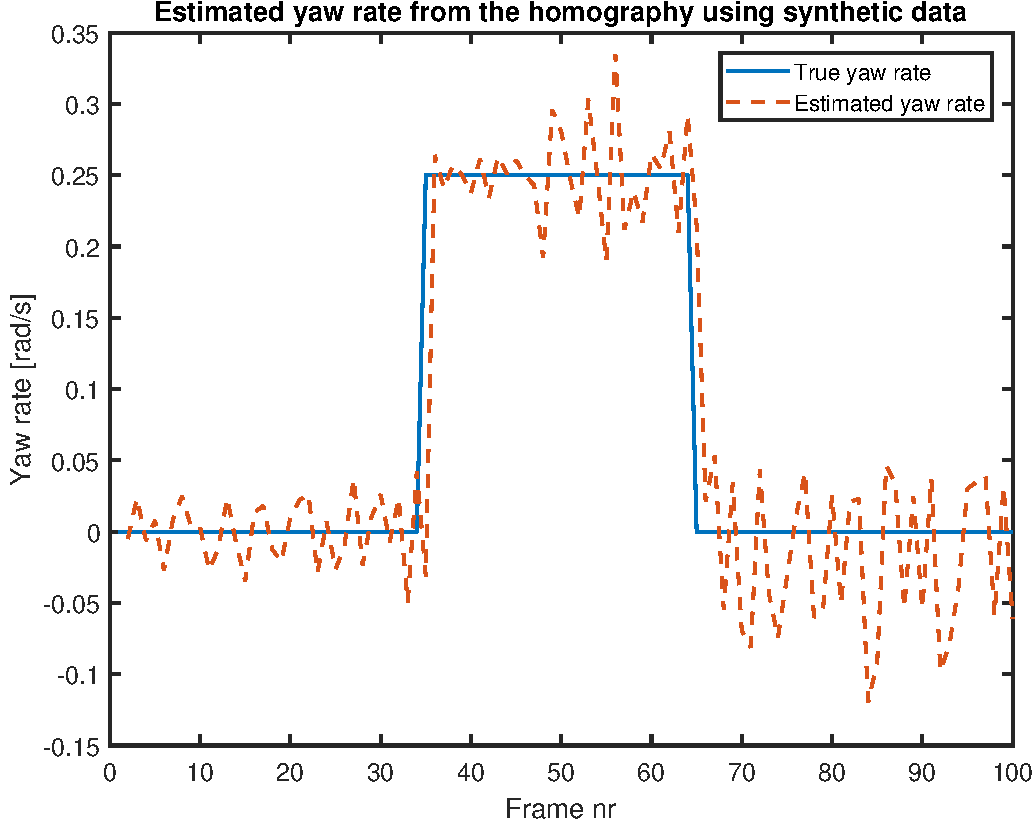
\includegraphics[height=0.35\textheight]{Hom/rect_1e-2}
		\vspace{-1.25em}
		\caption{Standard deviation 0.01 [px].}
	\end{figure}
	\vspace{-2.5em}
	\begin{figure}
		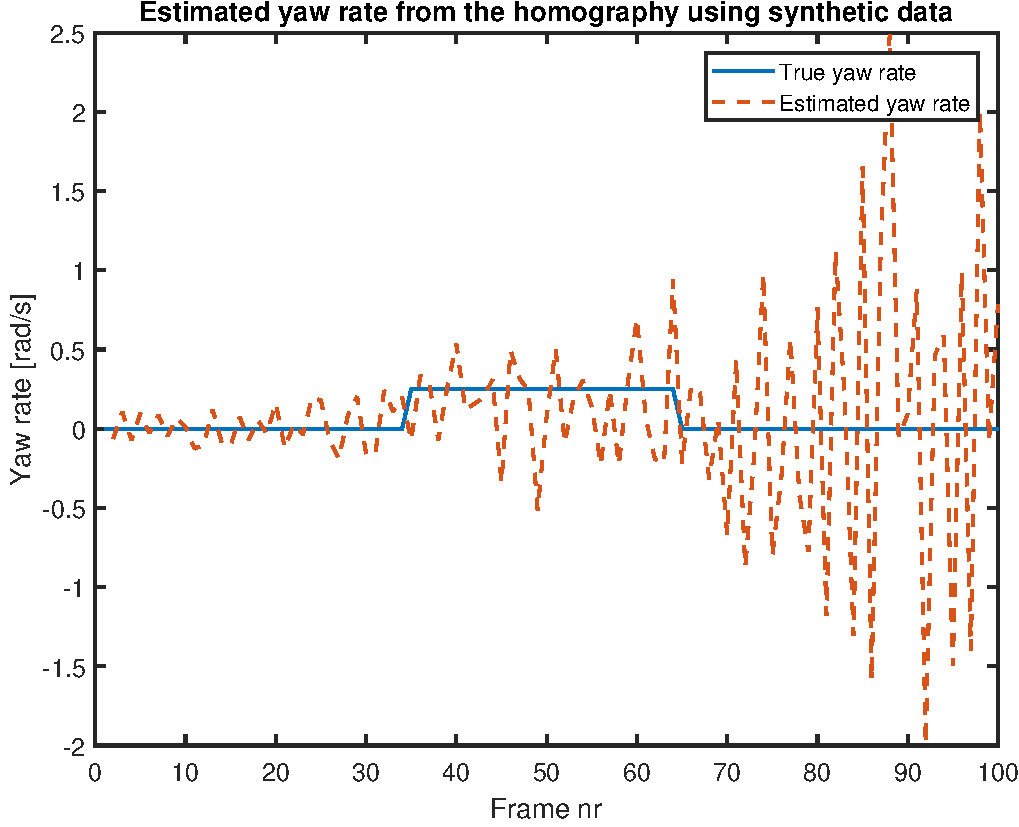
\includegraphics[height=0.35\textheight]{Hom/rect_1e-1}
		\vspace{-1.25em}
		\caption{Standard deviation 0.1 [px].}
	\end{figure}
	\column{0.45\textwidth}
	\begin{figure}
		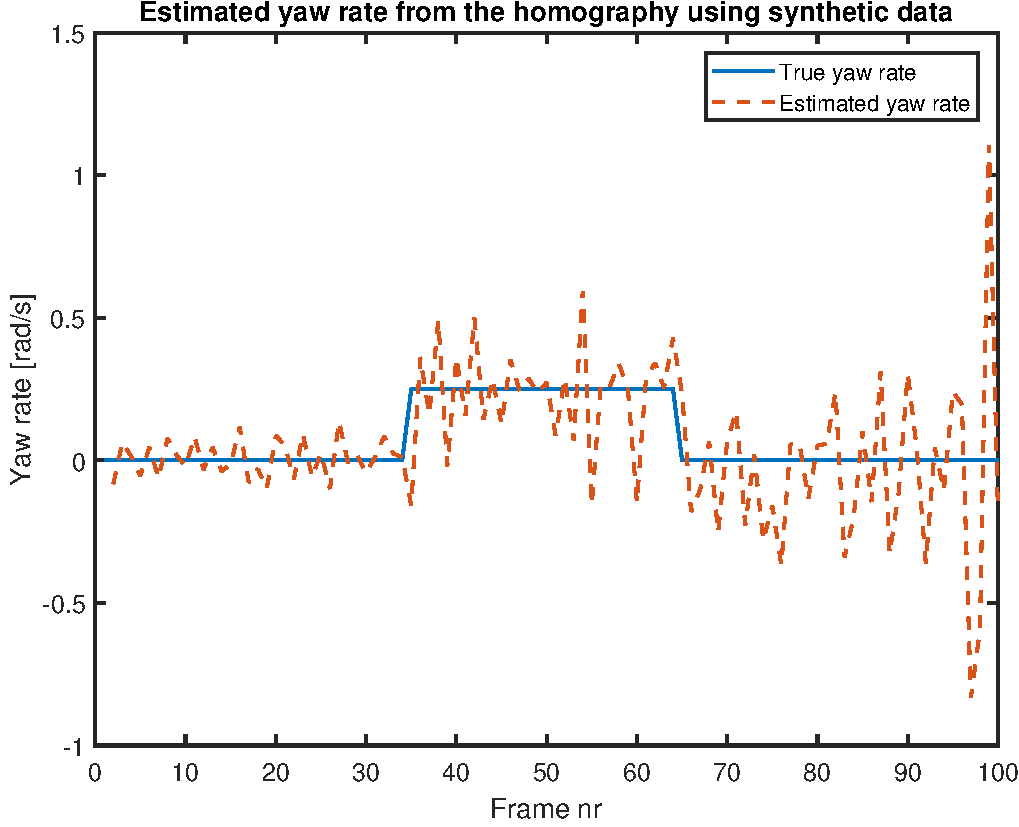
\includegraphics[height=0.35\textheight]{Hom/rect_5e-2}
		\vspace{-1.25em}
		\caption{Standard deviation 0.05 [px].}
	\end{figure}
	\vspace{-2.5em}
	\begin{figure}
		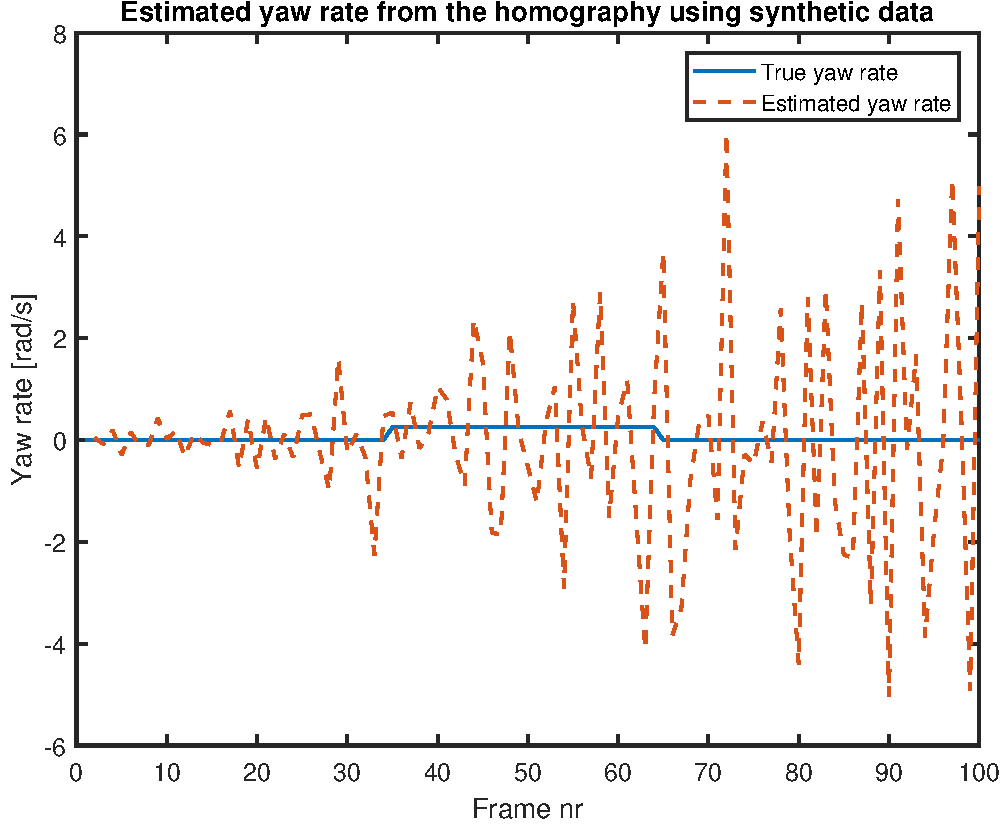
\includegraphics[height=0.35\textheight]{Hom/rect_5e-1}
		\vspace{-1.25em}
		\caption{Standard deviation 0.5 [px].}
	\end{figure}
	\end{columns}

	\note
	{
		\begin{itemize}
			\item Simulerad sv\aa{}ng m.h.a. trackade feature punkter innanf\o{}r en rektangel
			\vspace{2em}
			\item Additativt brus vid projicering till bildplanet
			\item Tyv\aa{}r verkar metoden vara brusk\aa{}nslig
			\item S\a{}mre p\a{} l\aa{}ngre avst\a{}nd
		\end{itemize}
	}
\end{frame}

\begin{frame}{Homography Estimation Results -- Real-world Data}
	\begin{columns}[T]
	\column{0.45\textwidth}
	\begin{figure}
		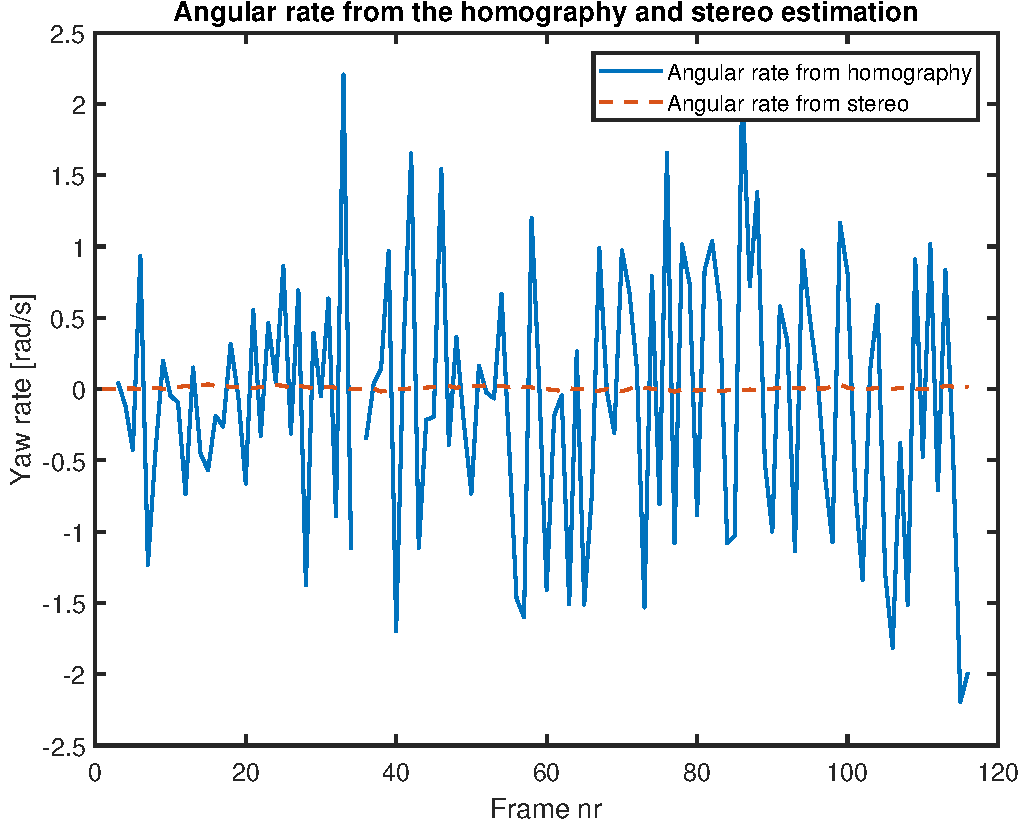
\includegraphics[width=\textwidth]{Hom/155532_AngVelComparison}
		\caption{Target driving straight and has a variance of 0.8 rad/s on the angular rate data.}
	\end{figure}
	\column{0.45\textwidth}
	\begin{figure}
		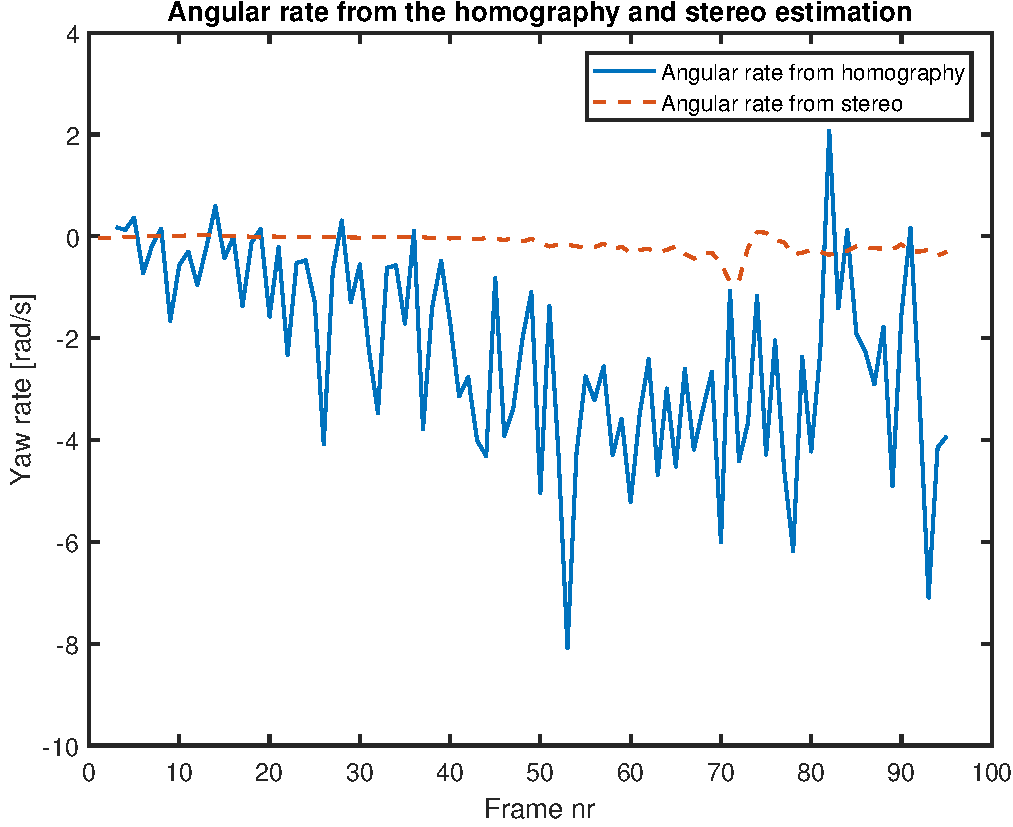
\includegraphics[width=\textwidth]{Hom/155733_AngVelComparison}
		\caption{Target turning right and has a variance of  2 rad/s on the angular rate data.}
	\end{figure}
	\end{columns}

	\note
	{
		\begin{itemize}
			\item \textit{F\o{}rsta sekvensen}

			Hyffsat okej skattning med lite f\o{}r stor varians

			\item \textit{Andra sekvensen}

			\"Overskattar sv\aa{}ngen och har f\o{}r stor varians

			\vspace{2em}
			\item F\o{}rb\aa{}ttra feature punkt f\o{}ljningen
			\item Utveckla homografiskattningsmetoden
			\item Fundamental begr\aa{}nsning -- Avst\a{}ndet till targetbilen?
		\end{itemize}
	}
\end{frame}

\begin{frame}<presentation:0>[noframenumbering]
	\frametitle{Homography Estimation Results -- Veoneer's FPM (1)}
	The target is driving straight.
	\begin{columns}
	\column{0.45\textwidth}
	\begin{figure}
		\centering
		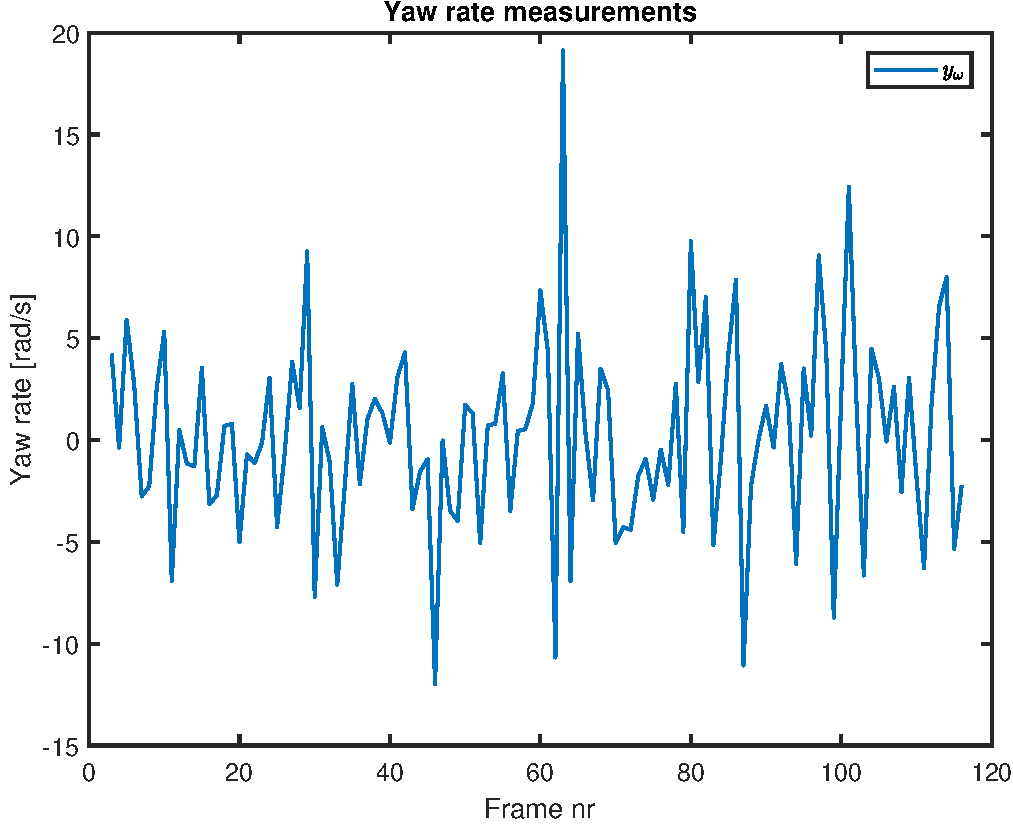
\includegraphics[width=\textwidth]{Veoneer/155532_AngVel_NoGate_fpm}
		\caption{Non pre-processed angular rate measurements. The variance is 22 rad/s.}
	\end{figure}
	\column{0.45\textwidth}
	\begin{figure}
		\centering
		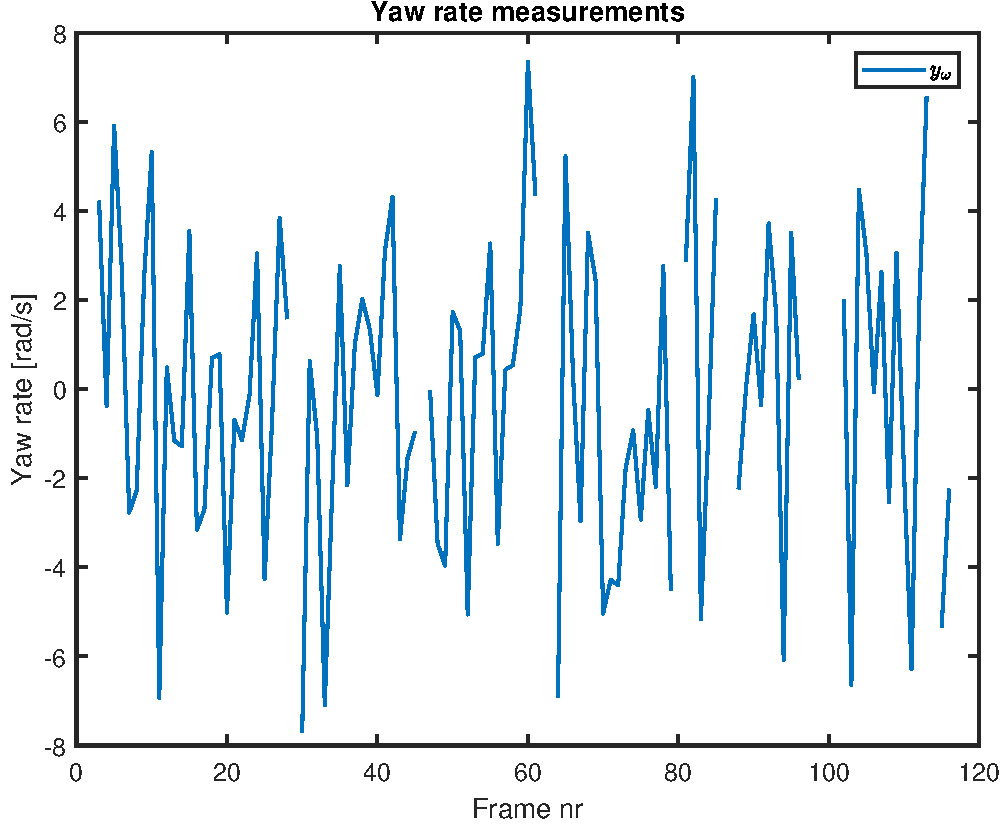
\includegraphics[width=\textwidth]{Veoneer/155532_AngVelMeasurements}
		\caption{Pre-processed angular rate measurements. The variance is 12 rad/s.}
	\end{figure}
	\end{columns}

	\note
	{
		\begin{itemize}
			\item Pre-processed: measurements rejected by the measurement gate and threshold at $|\}omega|<10$ rad/s.
		\end{itemize}
	}
\end{frame}

\begin{frame}<presentation:0>[noframenumbering]
	\frametitle{Homography Estimation Results -- Veoneer's FPM (2)}
	The target is turning to the right.
	\begin{columns}
	\column{0.45\textwidth}
	\begin{figure}
		\centering
		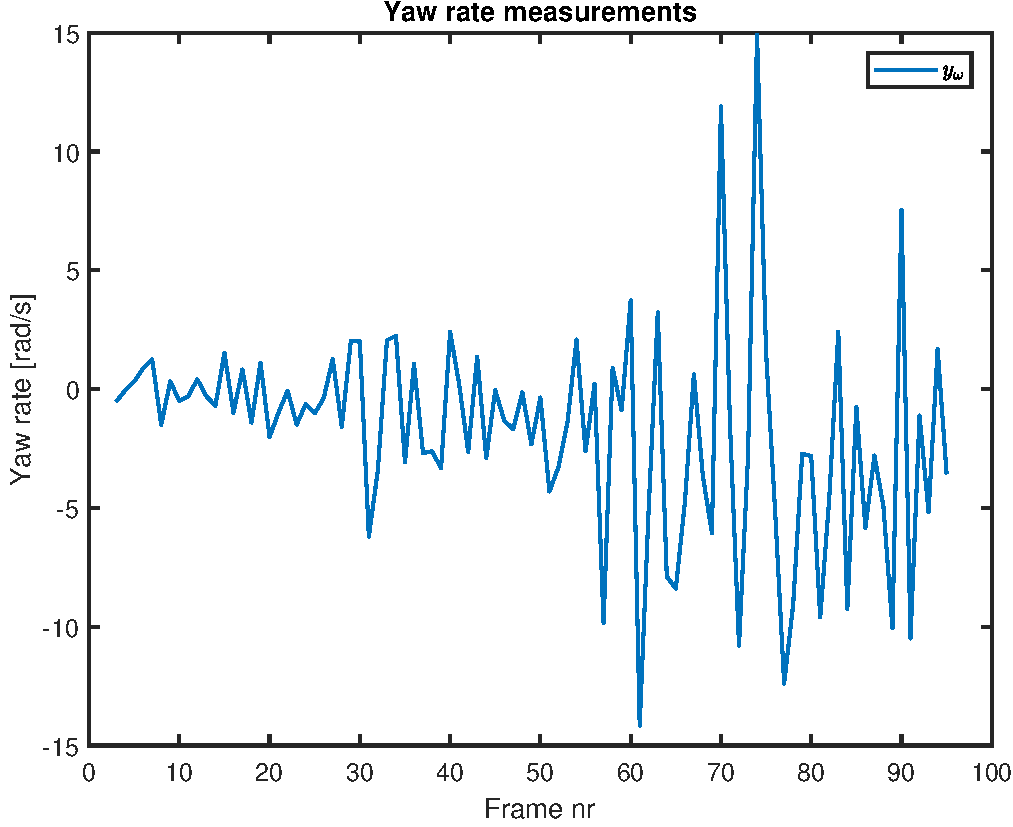
\includegraphics[width=\textwidth]{Veoneer/155733_AngVel_NoGate_fpm}
		\caption{Non pre-processed angular rate measurements. The variance is 17 rad/s.}
	\end{figure}
	\column{0.45\textwidth}
	\begin{figure}
		\centering
		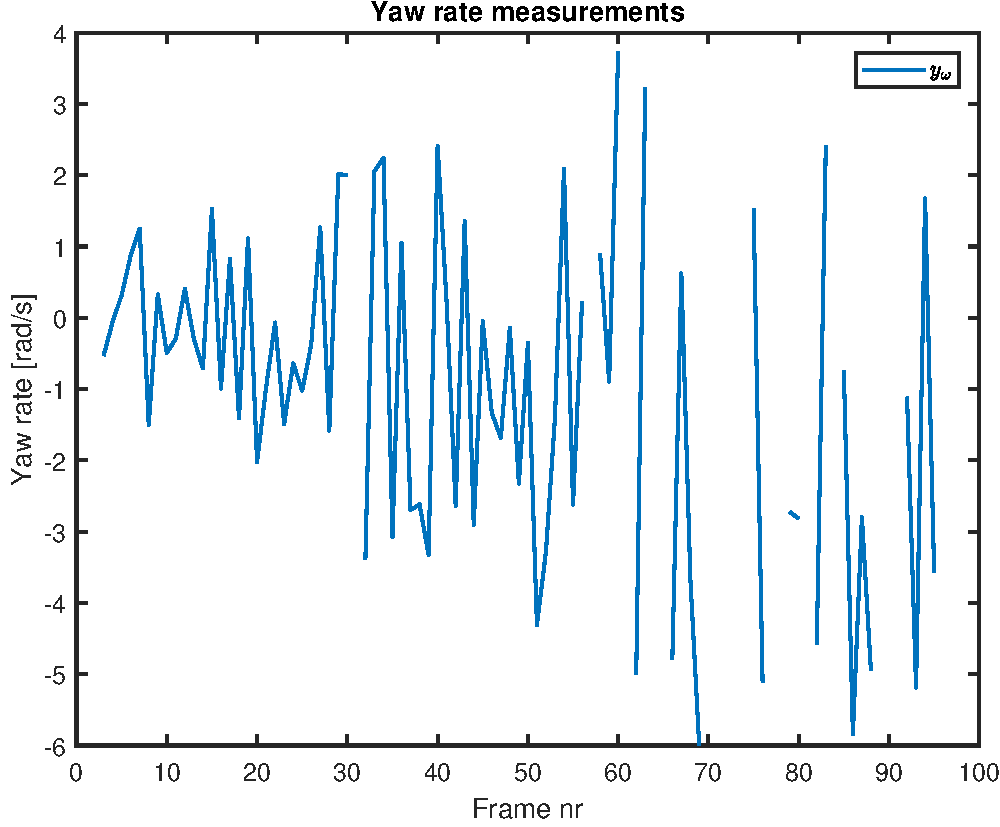
\includegraphics[width=\textwidth]{Veoneer/155733_AngVelMeasurements}
		\caption{Pre-processed angular rate measurements. The variance is 5 rad/s.}
	\end{figure}
	\end{columns}

	\note
	{
		\begin{itemize}
			\item Pre-processed: measurements rejected by the measurement gate and threshold at $|\}omega|<10$ rad/s.
		\end{itemize}
	}
\end{frame}

\subsection{Stereo Comparison}

\begin{frame}{Stereo Comparison -- No. 1}
	The target is driving straight.
	\begin{columns}[T]
	\column{0.45\textwidth}
	\begin{figure}
		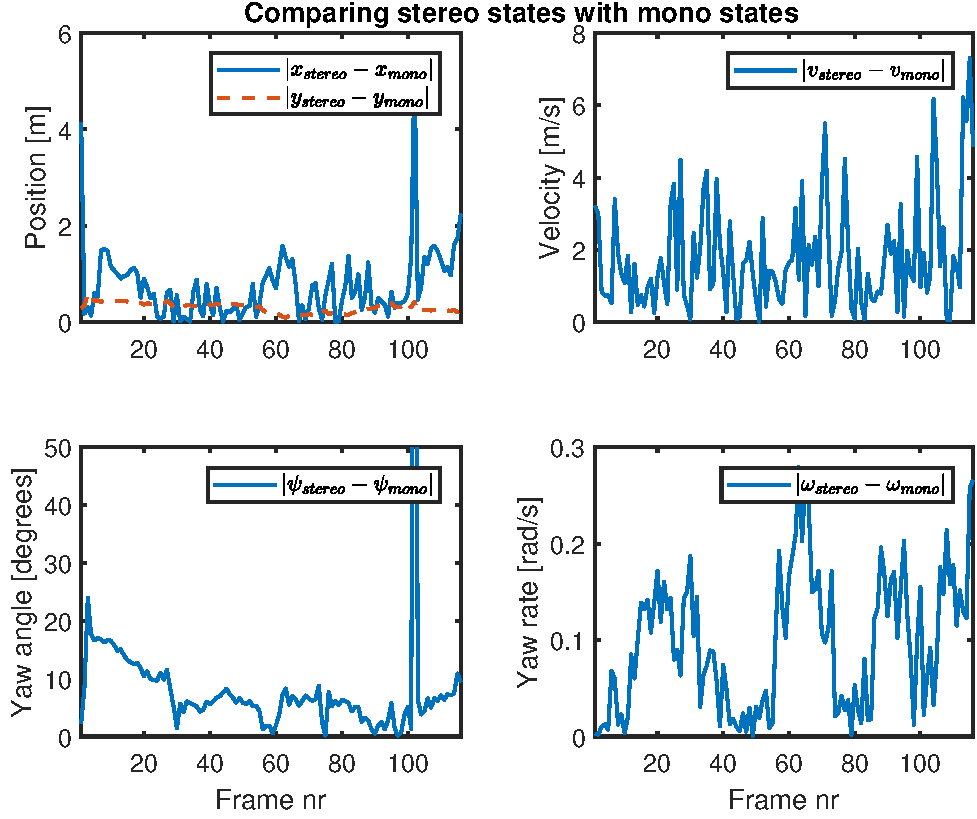
\includegraphics[width=\textwidth]{Stereo/155532_RoiAngVel_gate_klt}
		\caption{\roi and angular rate measurements.}
	\end{figure}
	\column{0.45\textwidth}
	\begin{figure}
		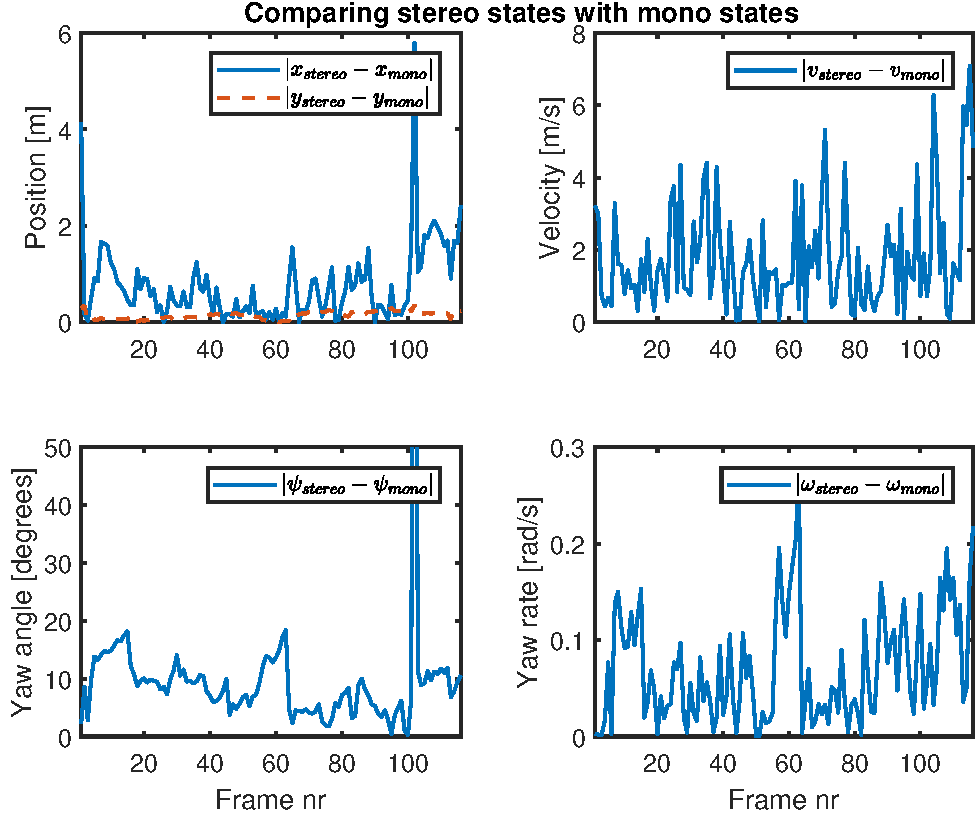
\includegraphics[width=\textwidth]{Stereo/155532_AllMeasurements_gate_klt}
		\caption{\roi, angular rate and corner measurements.}
	\end{figure}
	\end{columns}

	\note
	{
		\begin{itemize}
			\item Ingen signifikant f\o{}rb\aa{}ttring när h\o{}rnm\aa{}tningar l\aa{}ggs till
		\end{itemize}
	}
\end{frame}

\begin{frame}<presentation:0>[noframenumbering]
	\frametitle{Stereo Comparison -- Veoneer's FPM (1)}
	The target is turning to the right.
	\begin{columns}
	\column{0.45\textwidth}
	\begin{figure}
		\centering
		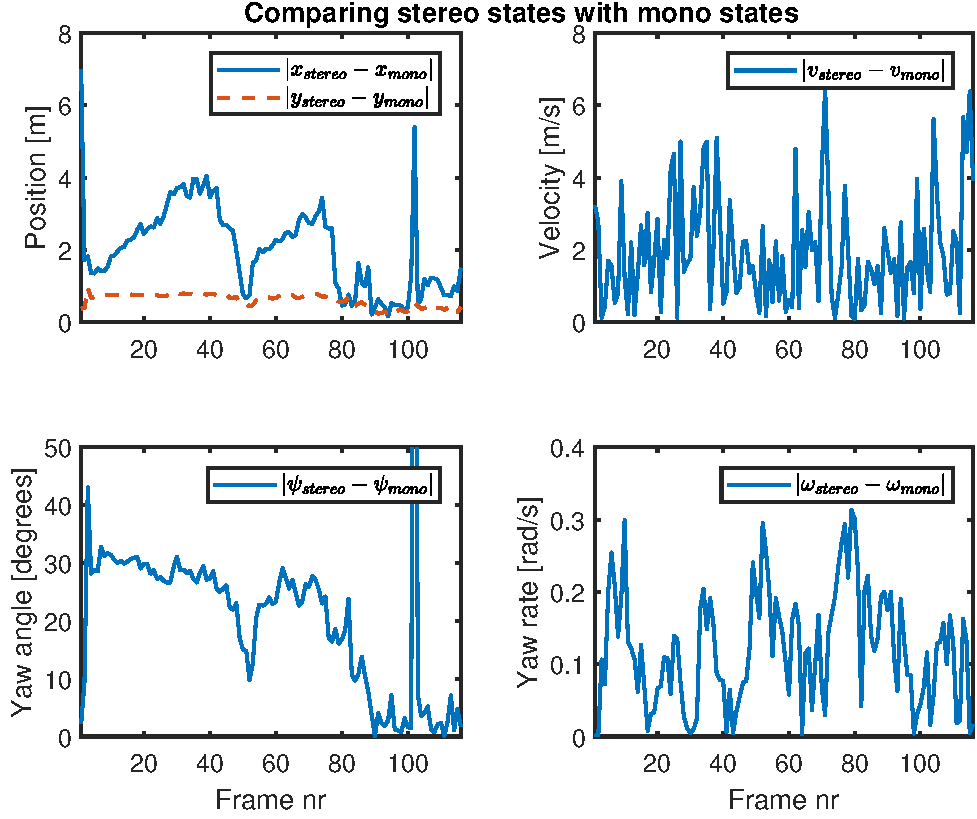
\includegraphics[width=\textwidth]{Veoneer/155532_RoiAngVel_gate}
		\caption{\roi and angular rate measurements.}
	\end{figure}
	\column{0.45\textwidth}
	\begin{figure}
		\centering
		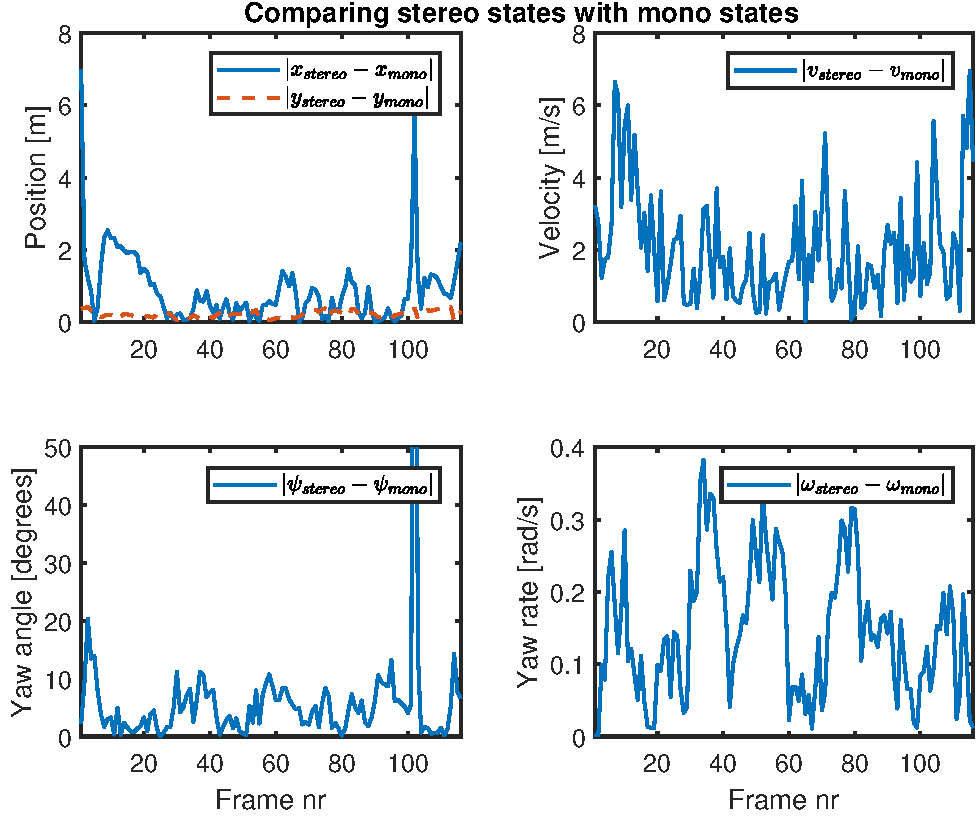
\includegraphics[width=\textwidth]{Veoneer/155532_AllMeasurements_gate}
		\caption{\roi, angular rate and corner measurements.}
	\end{figure}
	\end{columns}

	\note
	{
		\begin{itemize}
			\item Ganska skakigt resultat i orientering
			\item Stor f\o{}rb\aa{}tring med h\o{}rnm\aa{}tningar
		\end{itemize}
	}
\end{frame}

\begin{frame}{Stereo Comparison -- No. 2}
	The target is turning to the right.
	\begin{columns}[T]
	\column{0.45\textwidth}
	\begin{figure}
		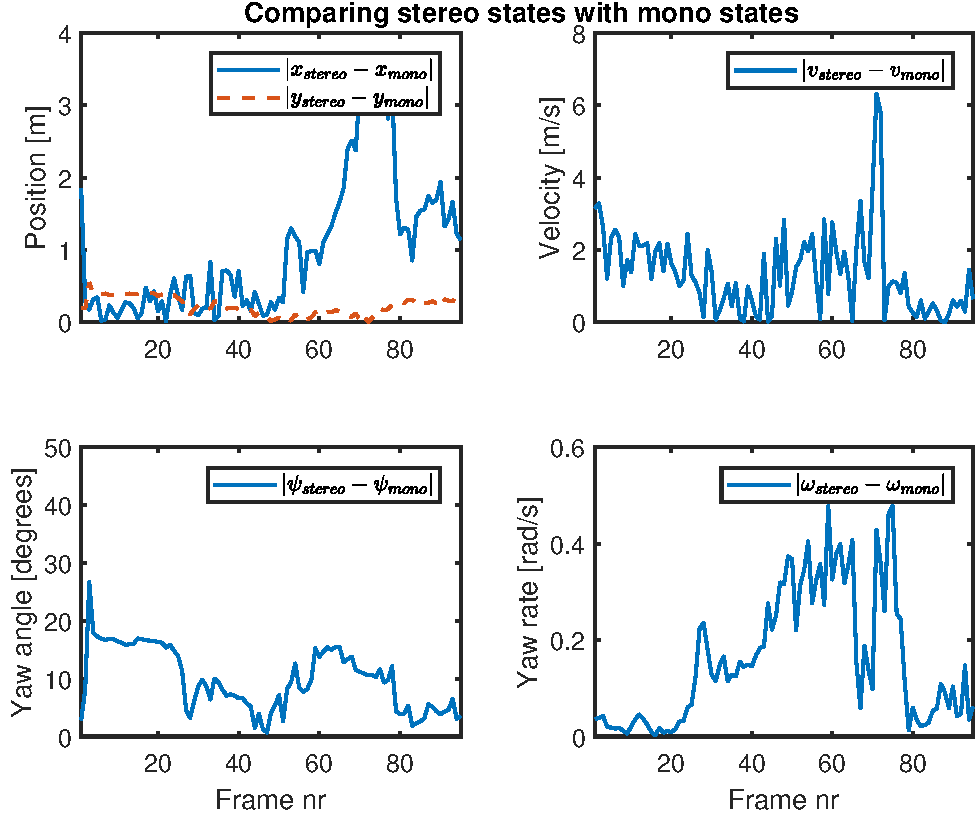
\includegraphics[width=\textwidth]{Stereo/155733_RoiAngVel_gate_klt}
		\caption{\roi and angular rate measurements.}
	\end{figure}
	\column{0.45\textwidth}
	\begin{figure}
		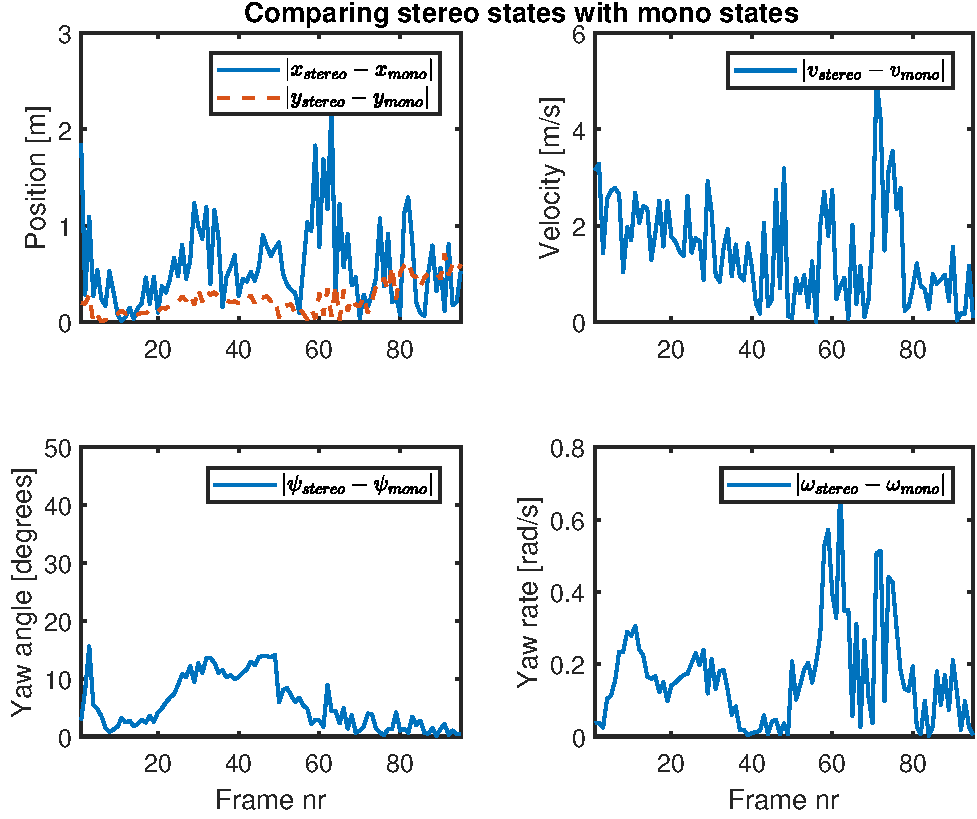
\includegraphics[width=\textwidth]{Stereo/155733_AllMeasurements_gate_klt_perf}
		\caption{\roi, angular rate and corner measurements.}
	\end{figure}
	\end{columns}

	\note
	{
		\begin{itemize}
			\item F\o{}rb\aa{}ttring i b\o{}rjan och i slutet
			\item 3 h\o{}rn synliga fr\a{}n frame nr. 60 -{}-$>$
			\item Ingen st\o{}rre f\o{}rb\aa{}ttring i vinkelhastighet, f\o{}r d\a{}liga m\aa{}tningar?
		\end{itemize}
	}
\end{frame}

\begin{frame}<presentation:0>[noframenumbering]
	\frametitle{Stereo Comparison -- Veoneer's FPM (2)}
	The target is turning to the right.
	\begin{columns}
	\column{0.45\textwidth}
	\begin{figure}
		\centering
		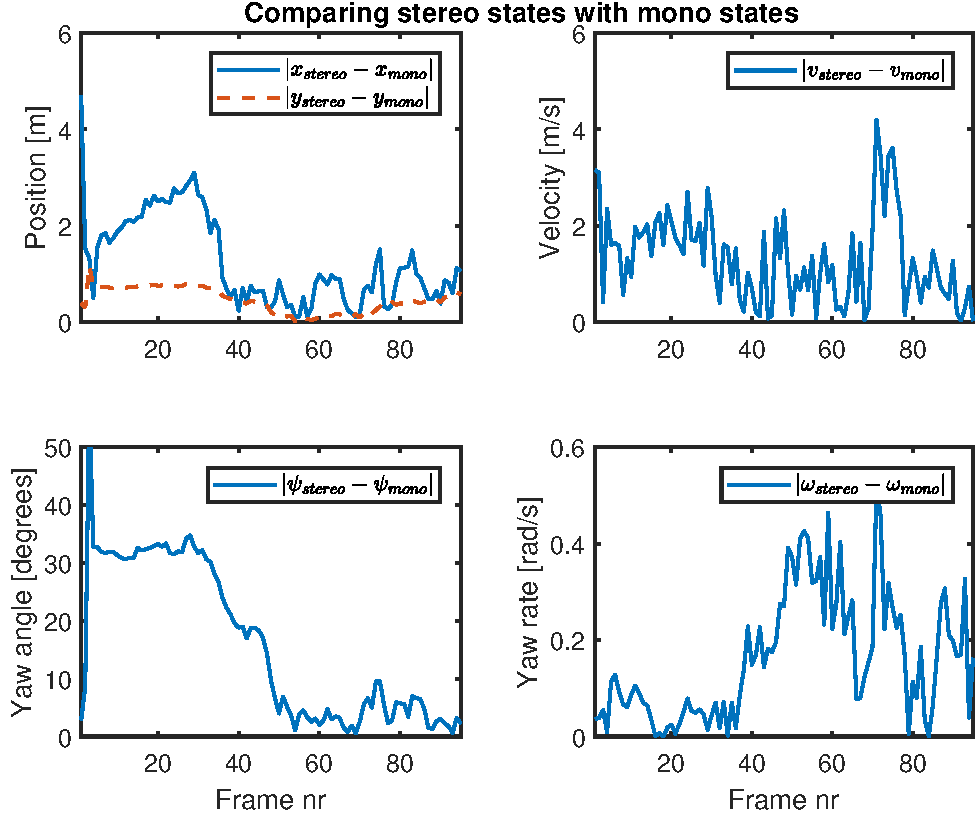
\includegraphics[width=\textwidth]{Veoneer/155733_RoiAngVel_gate}
		\caption{\roi and angular rate measurements.}
	\end{figure}
	\column{0.45\textwidth}
	\begin{figure}
		\centering
		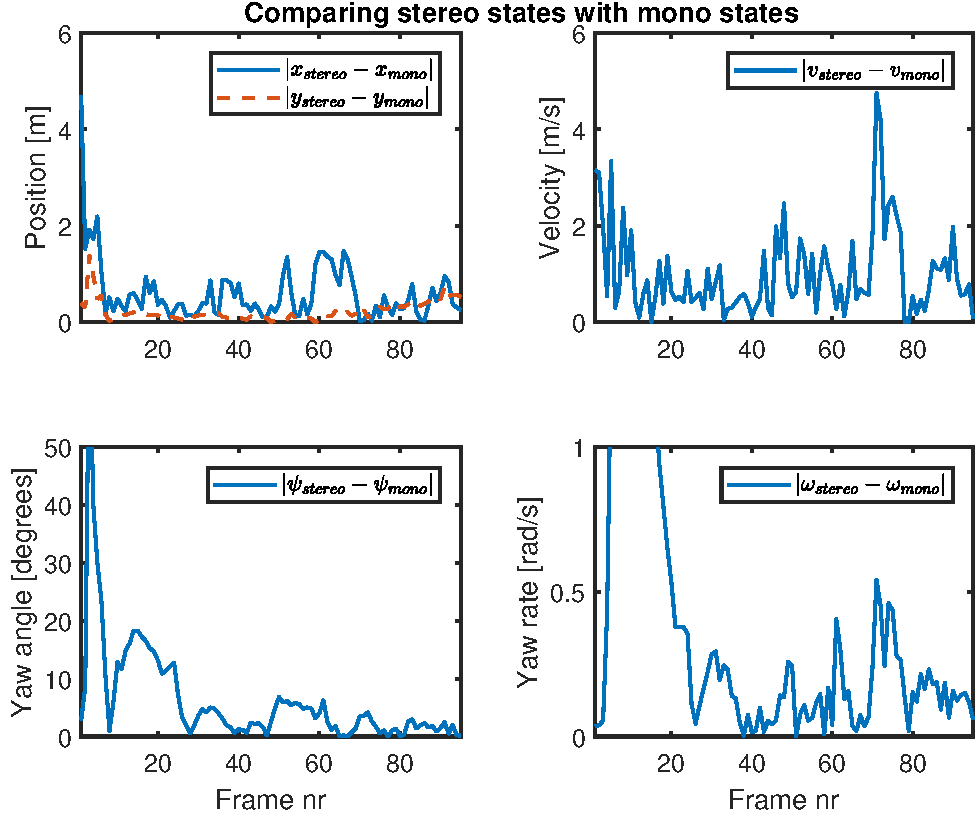
\includegraphics[width=\textwidth]{Veoneer/155733_AllMeasurements_gate}
		\caption{\roi, angular rate and corner measurements.}
	\end{figure}
	\end{columns}

	\note
	{
		\begin{itemize}
			\item Ganska skakigt resultat i orientering
			\item Stor f\o{}rb\aa{}tring med h\o{}rnm\aa{}tningar
		\end{itemize}
	}
\end{frame}

% -------------------
\section{Conclusions}
% -------------------

\begin{frame}{Conclusions}
	\begin{itemize}
		\item The heading can be estimated
		\begin{itemize}
			\item given the proper measurements,
			\item with high enough accuracy.
		\end{itemize}
		\item The extended Kalman filter is a suitable filter structure.
		\item Still some performance difference compared to stereo.
	\end{itemize}

	\note
	{
		\begin{itemize}
			\item Ganska h\o{}ga krav p\a{} m\aa{}tningarnas noggrannhet
			\item Utifr\a{}n simuleringarna verkar metoden (\ekf med rektangel model) fungera v\aa{}l
			\item Fortfarande en bit kvar till stereo prestanda, speciellt i vinkelhastighet
			\vspace{2em}
			\item Utveckla homografiskattningsmetoden
			\item F\o{}rb\aa{}tra feature punkt f\o{}ljningen
			\item Skapa en h\o{}rndetektor
		\end{itemize}
	}
\end{frame}

\end{document}
